
%--------------- Personalize your document here ---------------

\author{Farimah Anvari} % Enter your name
%\authortwo{Sajedeh Firouzizadeh} % Enter your name
\newcommand{\authortwo}{Sajedeh Firouzizadeh}
\newcommand{\studentID}{10772192} % enter your student ID 10771435
\newcommand{\studentIDS}{10771435} % enter your student ID 
\newcommand{\supervisorone}{Prof. Elisabetta Di Nitto} % Enter your supervisor's name
\newcommand{\supervisortwo}{Prof. Matteo Rossi}% Leave it empty or enter your second supervisor's name 
\newcommand{\department}{Dipartimento di Elettronica, Informazione e Bioingegneria}
\newcommand{\exam}{Software Engineering II Project RASD}

\title{DREAM} %Enter the title of your report 
\version{2.0}
\date{December 2021} % insert a specific date	

%--------------------------------------------------------------

% This document was adapted from the
% TEMPLATE FOR PHYS250 WORKSHEET created by Alastair McLean
% URL: https://www.overleaf.com/latex/templates/phys250-worksheet-template/xxftvfhmwqdt

% Jefferson Silveira
% Email: 19jdls1@queensu.ca
% Last update: 09-Jun-2021
% If you have any questions or concerns, do not hesitate to contact me.
%--------------------------------------------------------------

\documentclass[a4paper,12pt]{article}
\usepackage[left=30mm,top=30mm,right=30mm,bottom=30mm]{geometry}
\usepackage{etoolbox} %required for cover page
\usepackage{booktabs}
\usepackage[usestackEOL]{stackengine}
\usepackage[T1]{fontenc}
\usepackage[utf8]{inputenc}
\usepackage{bm}
\usepackage{graphicx}
\usepackage{float}

\usepackage[table,xcdraw]{xcolor}
\definecolor{tableBorderColor}{rgb}{.5,.5,.5}
\definecolor{tableHighlightColor}{rgb}{.8,.8,.8}
\definecolor{purpleHiglight}{rgb}{.63,.63,.76}
\definecolor{pinkHighlight}{rgb}{.95,.77, .88}

\usepackage{tabularx}
\usepackage{longtable}

\usepackage{float} 



\usepackage{subcaption}
\usepackage{amsmath}
\usepackage{amsfonts}
\usepackage{mathtools}
\usepackage{xcolor}
\usepackage{float}
\usepackage{hyperref}
\usepackage[capitalise]{cleveref}
\usepackage{enumitem,kantlipsum}
\usepackage{amssymb}
\usepackage[square,numbers,sort]{natbib}
\usepackage[ruled,vlined]{algorithm2e}
\usepackage{listings}
\usepackage{minted}
\usemintedstyle{emacs}

\renewcommand{\listingscaption}{Algorithm}
\renewcommand{\listoflistingscaption}{List of Algorithms}


\bibliographystyle{unsrtnat}

\hypersetup{
    colorlinks,
    linkcolor={black},
    citecolor={blue!50!black},
    urlcolor={blue!80!black}
}

\linespread{1}

\newtheorem{theorem}{Theorem}[section]
\graphicspath{{figures/}}	

%----------------------------------TITLE PAGE -----------------------------------
\makeatletter
\def\maketitle{
  \begin{center}\leavevmode
       \normalfont
       
\includegraphics[width=0.7\columnwidth]{poli_milano_logo.png}
       \vskip 0.5cm   
       \textsc{\large \department}\\
       \vskip 1.5cm
       \rule{\linewidth}{0.2 mm} \\
       {\large \exam}\\[1 cm]
       {\huge \bfseries \@title \par}
       \vspace{1cm}
	\rule{\linewidth}{0.2 mm} \\[1.5 cm]
	 
	\begin{minipage}[t]{0.45\textwidth}
		\begin{flushleft} \large
			\emph{Authors:}\\
			\@author: \studentID\\
			\authortwo:	\studentIDS
		\end{flushleft}
	\end{minipage}
	\begin{minipage}[t]{0.45\textwidth}
	    \begin{flushright} \large
			\ifdefempty{\supervisortwo}{\emph{Supervisor:\\}}{\emph{Supervisors:\\}}
			\supervisorone\\
			\ifdefempty{\supervisortwo}{}{\supervisortwo\\}
		\end{flushright}
	\end{minipage}
	\vfill
	{\Large \@date\par}
   \end{center}
   %\vfill
   %\null
   %\cleardoublepage
  }
\makeatother


%-------------------------------- ENDTITLE PAGE ----------------------------------

\begin{document}

\pagenumbering{gobble}% Remove page numbers (and reset to 1)

\maketitle
\clearpage
\tableofcontents
\newpage
%\listoffigures
%\newpage
%\listoftables
%\newpage
%\listofalgorithms % List of algorithms in pseudocode format
%\newpage
%\listoflistings % List of algorithms in code format
%\newpage


\pagenumbering{arabic}% Arabic page numbers (and reset to 1)

% This is how you can organize your document
\section{Introduction}

\subsection{Purpose}
\paragraph{}
This is the Design Document (DD) of DREAM application. The purpose of this document is to discuss more technical aspects regarding architectural and design choices that must be made, so as to follow well-oriented implementation and testing processes. This document is to provide more technical and detailed information about the software discussed in the RASD document.\\
In this DD we present hardware and software architecture of the system in terms of components and interactions among those components. Furthermore, this document describes a set of design characteristics required for the implementation by introducing constraints and quality attributes.
It also gives a detailed presentation of the implementation plan, integration plan and the testing plan.\\
In this document we mostly talk about:
\begin{itemize}
    \item The High-level architecture of the system.
    \item Main components of the system.
    \item Interfaces provided by the components.
    \item Design patterns.
    \item final representation 
\end{itemize}

\subsection{Scope}

The software wants give them the possibility to see the details of their lands and the predictions, start discussions and ask their problems.
\paragraph{Basic service} Farmers can visualize data relevant to them and also allow farmers to follow the progress of their lands and the details about the irrigation and products based on the information that the application gave them. Also, they can insert the data about their lands and also the updates about their products.
\paragraph{Advance Function1} Second functionality point out about the farmers that can create discussions with other farmers.  Also, they can insert any problem that they are faced.
\clearpage
\subsection{Definitions, Acronyms, Abbreviations}
\subsubsection{Definitions}
\vspace{0.5cm}
\arrayrulecolor{tableBorderColor}
\setlength\arrayrulewidth{1pt}
\rowcolors{2}{white}{tableHighlightColor}
\setlength\LTleft{0pt}
\begin{longtable}{ !\Vline l !\Vline l !\Vline}
    \hline
     \textbf{Policy Maker}   & A person who observe farmers progress\\
    \textbf{Farmers}        & A person who has a farm land on Telengana\\
    \textbf{Water-Irrigation System} & An organization who observe the amount of used water\\
    \textbf{Sensor}         & A device that sense a physical phenomena\\
    \hline
\end{longtable}

\subsubsection{Acronyms}

\arrayrulecolor{tableBorderColor}
\setlength\arrayrulewidth{1pt}
\rowcolors{2}{white}{tableHighlightColor}
\setlength\LTleft{0pt}
\begin{longtable}{ !\Vline l !\Vline l !\Vline}
    \hline
    \textbf{DD}     & Design Document\\
    \textbf{UI}     & User Interface\\
    \textbf{HTTP}   & Hypertext Transfer Protocol\\
    \textbf{HTTPS}   & Hypertext Transfer Protocol Over Secure Socket Layer\\
    \textbf{REST}   & Representation State Transfer\\
    \textbf{JSON}   & JavaScript Object Notation\\
    \textbf{RASD}   & Requirement Analysis and Specification Document\\
    \textbf{GPS}    & Global Positioning System\\
    \textbf{App}    & Application\\
    \textbf{API}    & Application Programming Interface\\
    \textbf{DBMS}    & Database Management System\\
    \textbf{ODBC}    & Open Database Connectivity\\
    \textbf{MVC}    & Model, View, Controller\\
    \textbf{SDK}    & Software Development Kit\\
    \hline
\end{longtable}

\subsubsection{Abbreviations}

\arrayrulecolor{tableBorderColor}
\setlength\arrayrulewidth{1pt}
\rowcolors{2}{white}{tableHighlightColor}
\setlength\LTleft{0pt}
\begin{longtable}{ !\Vline c !\Vline l !\Vline}
    \hline
    \textbf{BS}     & Basic Service of DREAM\\
    \textbf{AF1}    & Advance Function 1 of DREAM\\
    \textbf{Rn}     & Requirement number n\\
    \hline
\end{longtable}
\clearpage
\subsection{Revision history}

\arrayrulecolor{tableBorderColor}
\setlength\arrayrulewidth{1pt}
\rowcolors{2}{white}{tableHighlightColor}
\setlength\LTleft{0pt}
\begin{longtable}{ !\Vline c !\Vline l !\Vline}
    \hline
    \textbf{Date}   & \textbf{Modifications}\\
    \textbf{09/01/2021}     & First version\\
    % \textbf{23/12/2020}     & \begin{minipage} [t] {0.9\textwidth} 
    %   \begin{itemize}
    %   \item Adding alloy models and alloy code.
    %   \item Update Class Diagram.
    %   \item Adding Mockup images.
    %  \end{itemize} 
    %  \vspace{0.5em}
    % \end{minipage}
    \hline
\end{longtable}


\subsection{Reference Documents}

\begin{itemize}
    \item Specification Document: "R\&DD Assignment A.Y. 2021-2022.pdf"
    \item Slides of the lectures.
\end{itemize}

\subsection{Document Structure}
This document is divided in seven sections.
\begin{itemize}
    \item \textbf{Chapter 1} describes the scope and purpose of the DD, including the structure of the document and the set of definitions, acronyms and abbreviations used.
    
    \item \textbf{Chapter 2} contains the architectural design choice, it includes all the components, the interfaces, the technologies (both hardware and software) used for the development of the application. It also includes the main functions of the interfaces and the processes in which they are utilised (Runtime view and component interfaces). Finally, there is the explanation of the architectural patterns chosen with the other design decisions.
    
    \item \textbf{Chapter 3} shows how the user interface should be on the mobile and web application.
    
    \item \textbf{Chapter 4} describes the connection between the RASD and the DD, showing the matching between requirements described previously with the elements which compose the architecture of the application.
    
    \item \textbf{Chapter 5} traces a plan for the development of components to maximize the efficiency of the developer team and the quality controls team. It is divided in two sections: implementation and integration. It also includes the testing strategy.
    
    \item \textbf{Chapter 6} shows the effort spent for each member of the group.
    
    \item \textbf{Chapter 7} include the reference documents.
 \end{itemize}

\vfill

\clearpage
\input{sections/overall Description }
\section{Specific Requirements}
\subsection{External Interface Requirements}
    \subsubsection{User Interfaces}
    This application that we have should be able to receive information about each land and then track the progress of the farmers. We assume that each farmer signs up to our application and then inserts the data of the land, also we receive the forecasts of the meteorological data of Telangana. In these applications, farmers can create discussions and also ask about their problems. Policymakers can observe the farmland and choose the best and worst. There are notifications for farmers about the humidity, the amount of water that the land used, the forecast for weather in the app that helps them to improve their performance. You can see the mock up of our application in the following:
    
    \begin{figure}[H]
  \centering
  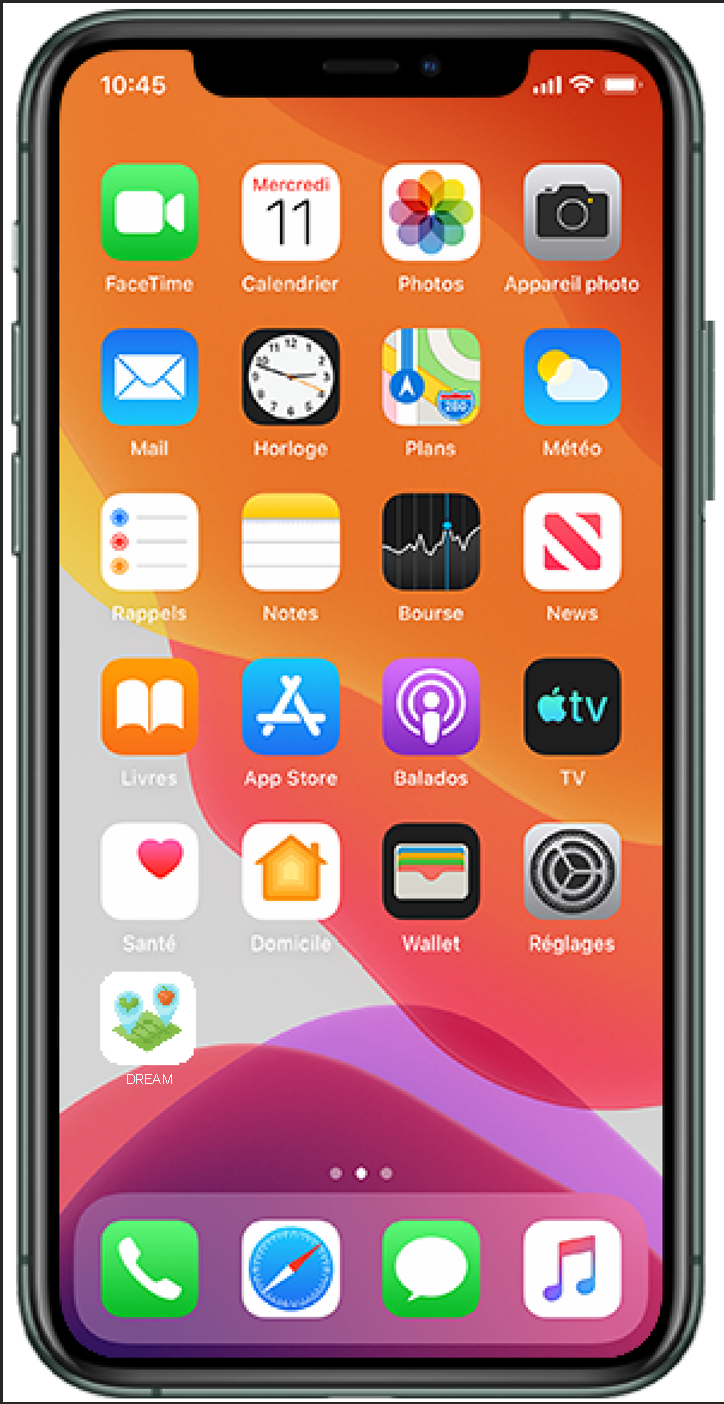
\includegraphics[width=0.5\textwidth,keepaspectratio]{figures/homescreen.png}
  \caption{App Icon}
\end{figure}
\begin{figure}[H]
  \centering
  \subfloat[Opening page] {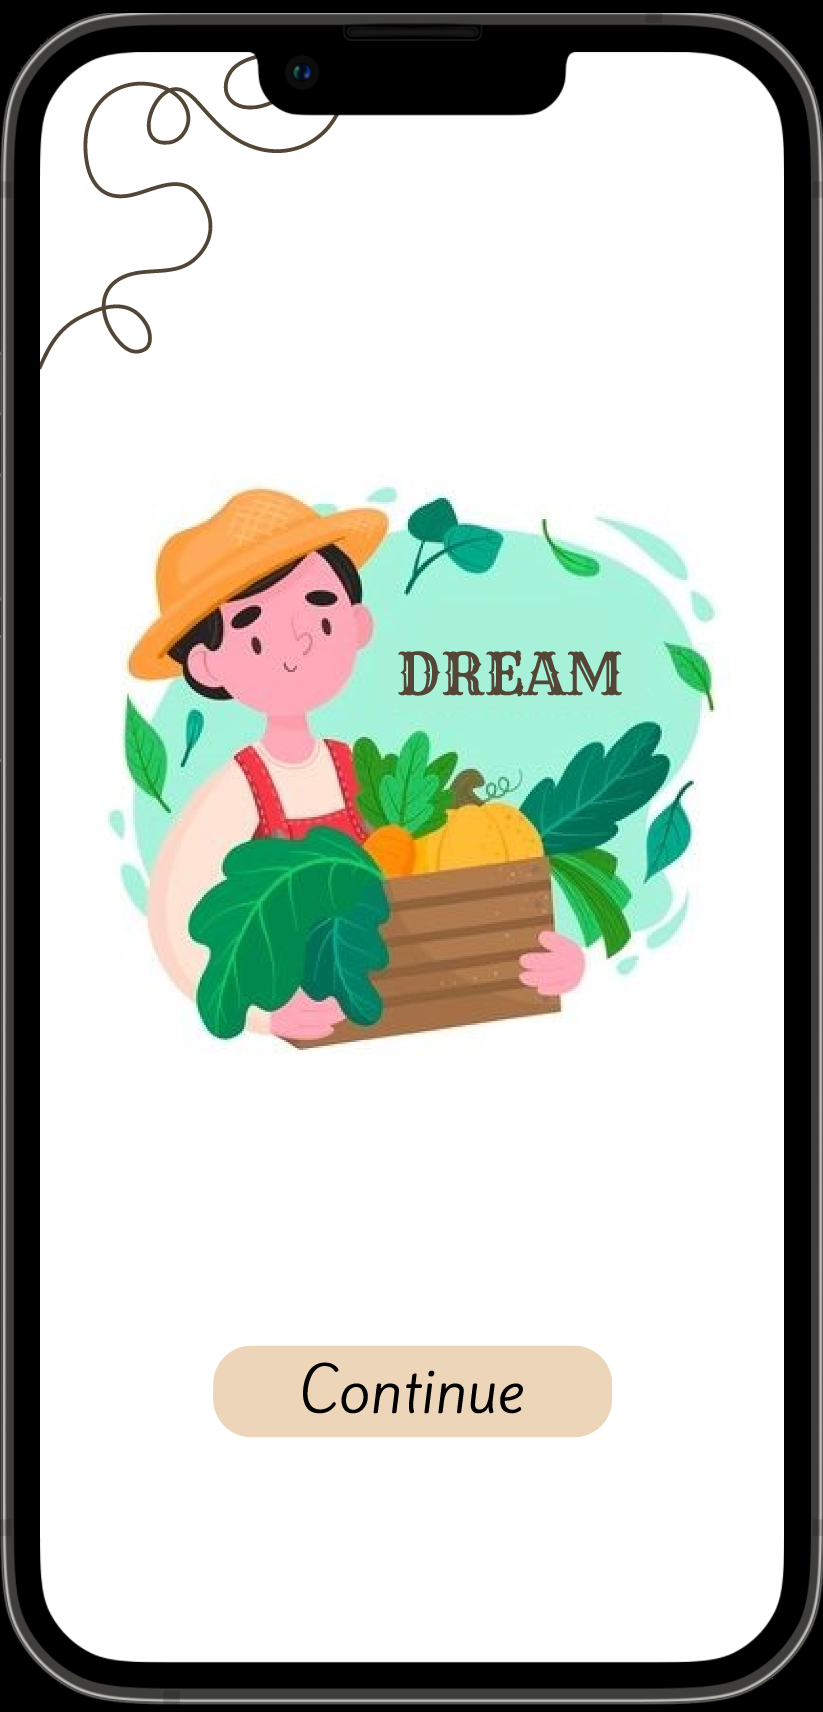
\includegraphics[width=0.4\textwidth,keepaspectratio]{figures/openning page.png}}
  \hfill
  \subfloat[sign in Farmers] {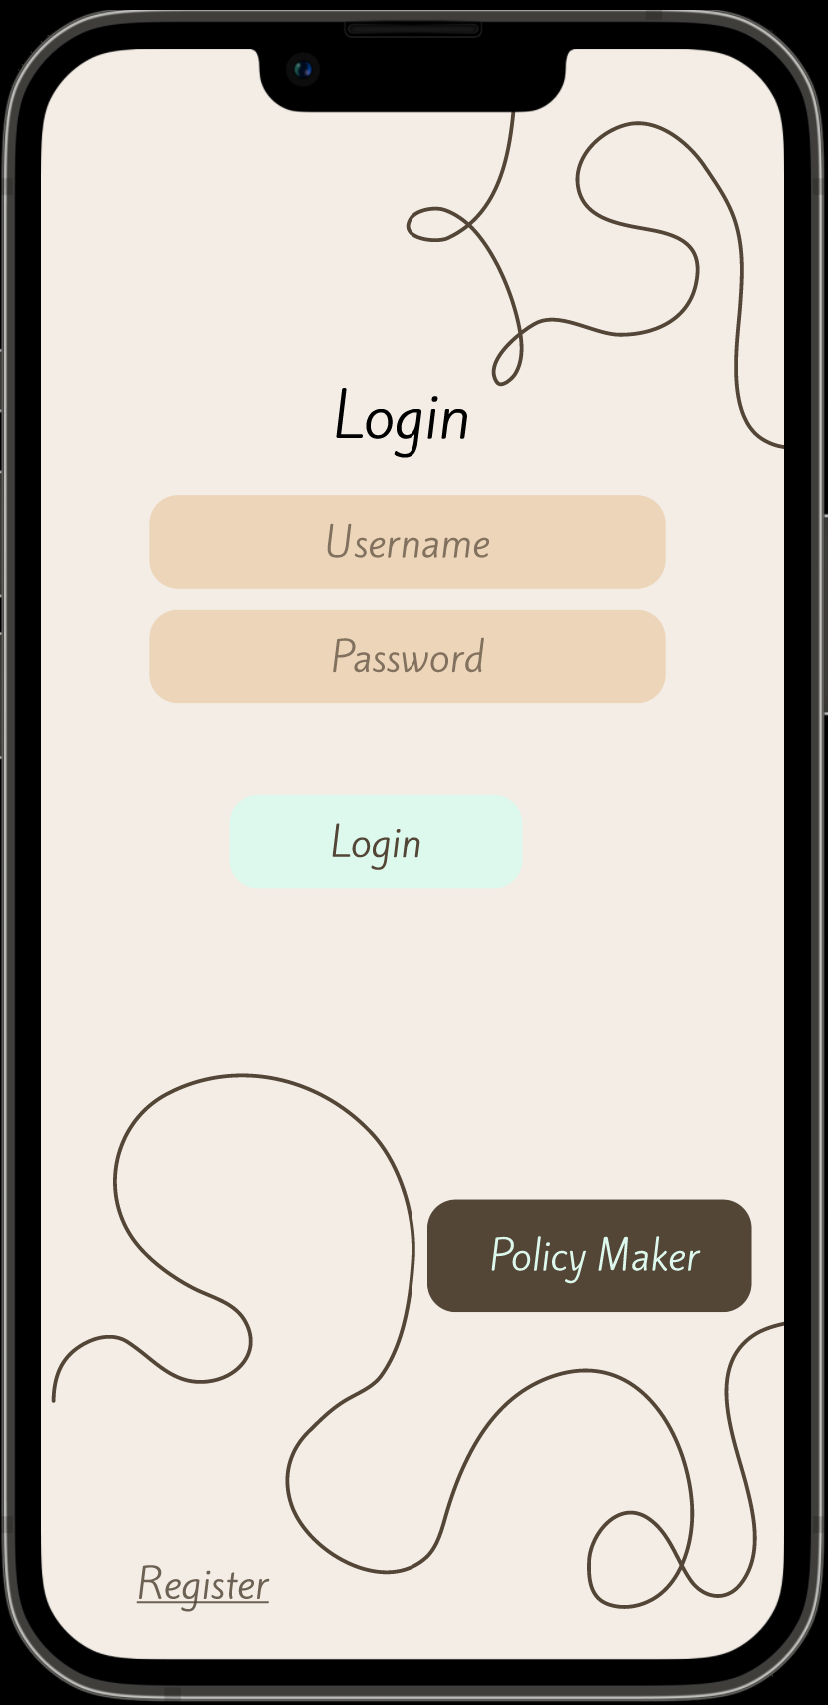
\includegraphics[width=0.4\textwidth,keepaspectratio]{figures/Loginpage.png}}
  \hfill
  \subfloat[sign in policy makers] {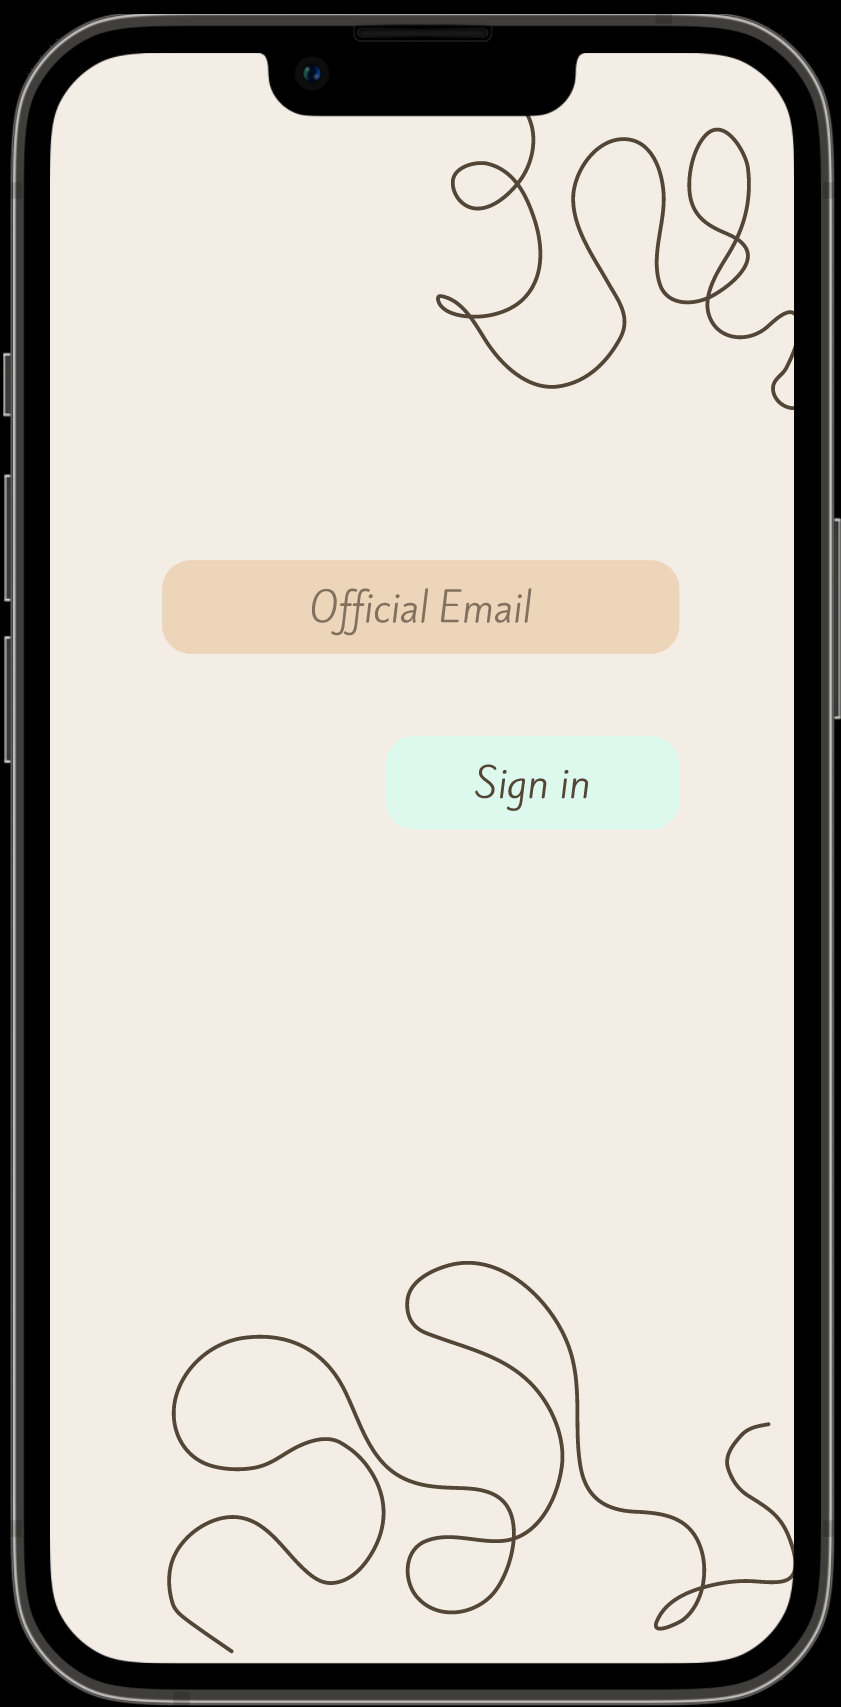
\includegraphics[width=0.4\textwidth,keepaspectratio]{figures/PolicymakerLogin.png}}
  \hfill
  \subfloat[sign up Farmers] {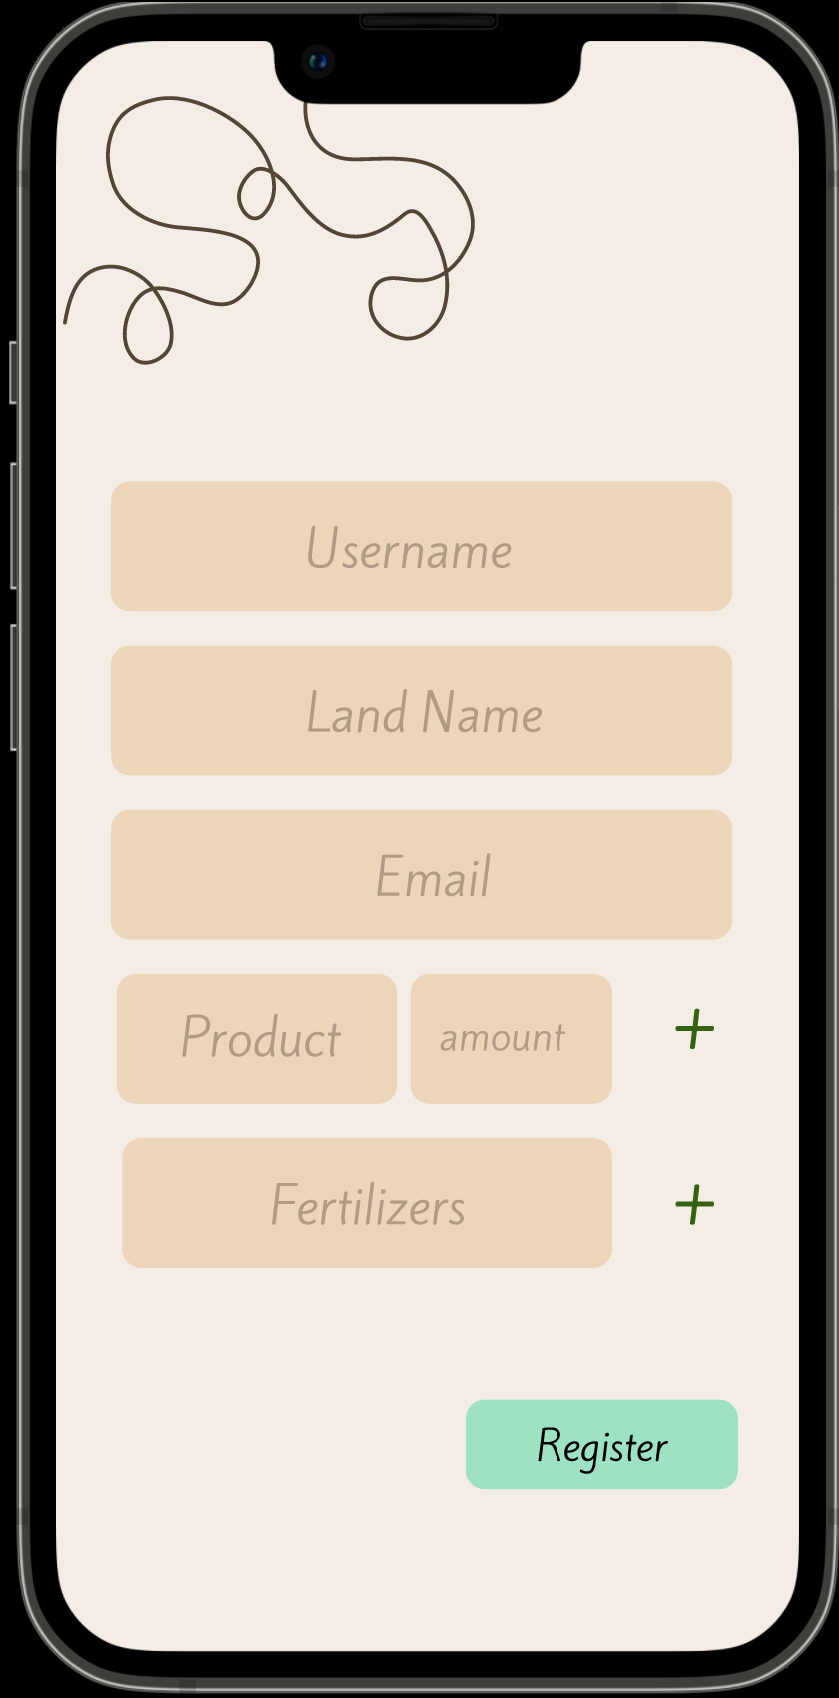
\includegraphics[width=0.4\textwidth,keepaspectratio]{figures/signupFarmers.png}}
  \hfill

  %\caption{Mockup}
\end{figure}
\begin{figure}[H]
  \centering
  
  \subfloat[Farmers Main page] {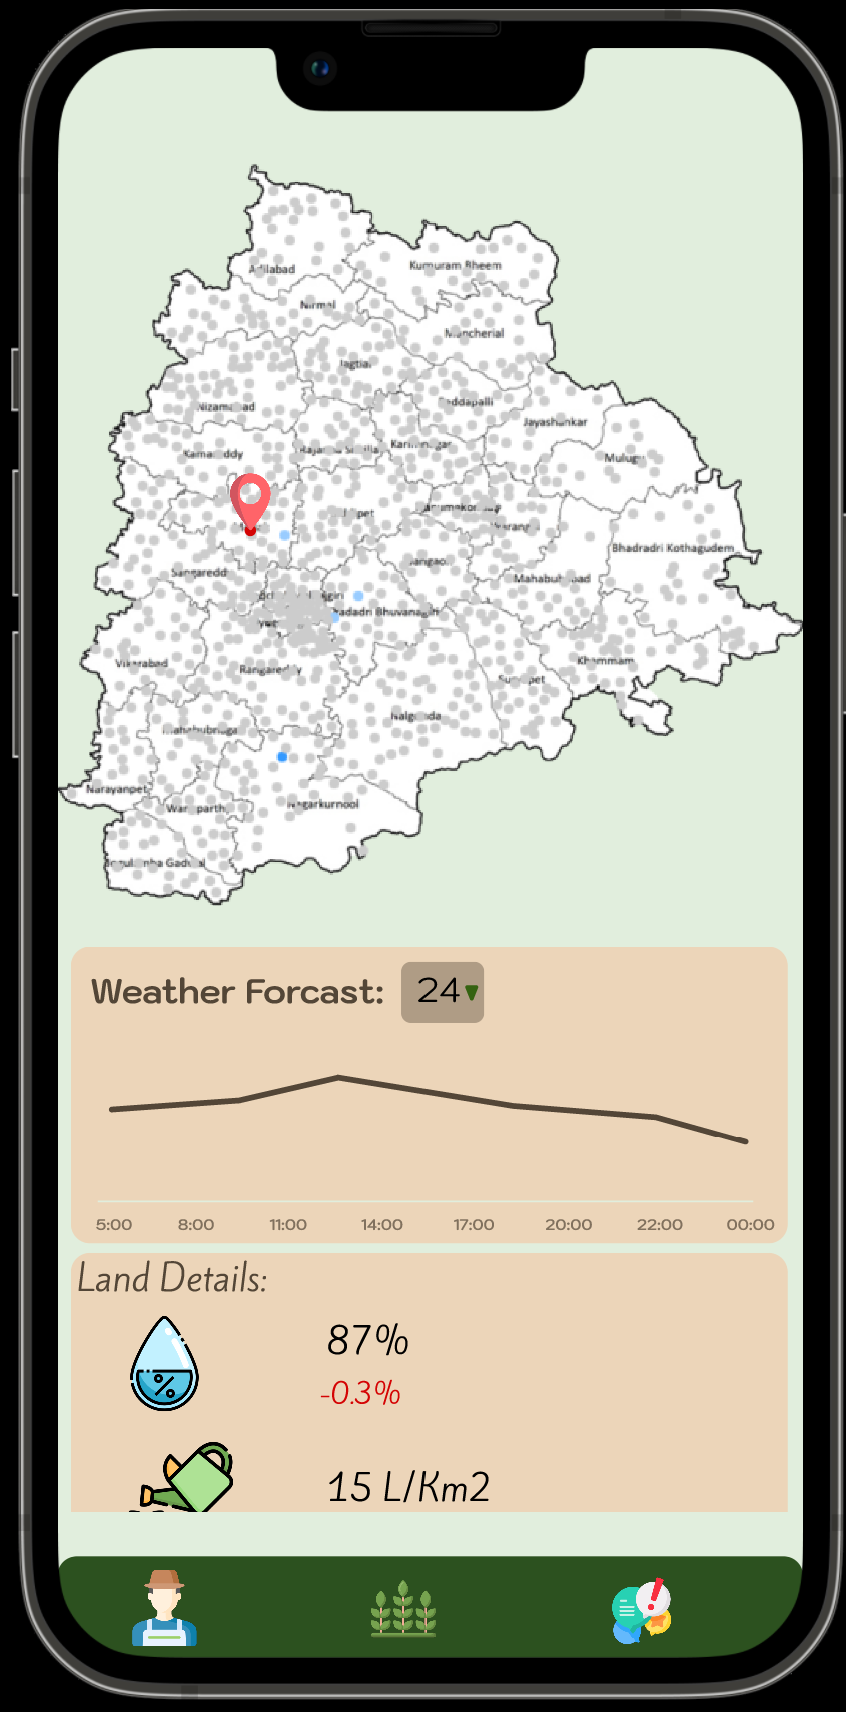
\includegraphics[width=0.4\textwidth,keepaspectratio]{figures/FarmersMainPage.png}}
  \hfill
  \hfill
  \subfloat[Policy-Makers Main page] {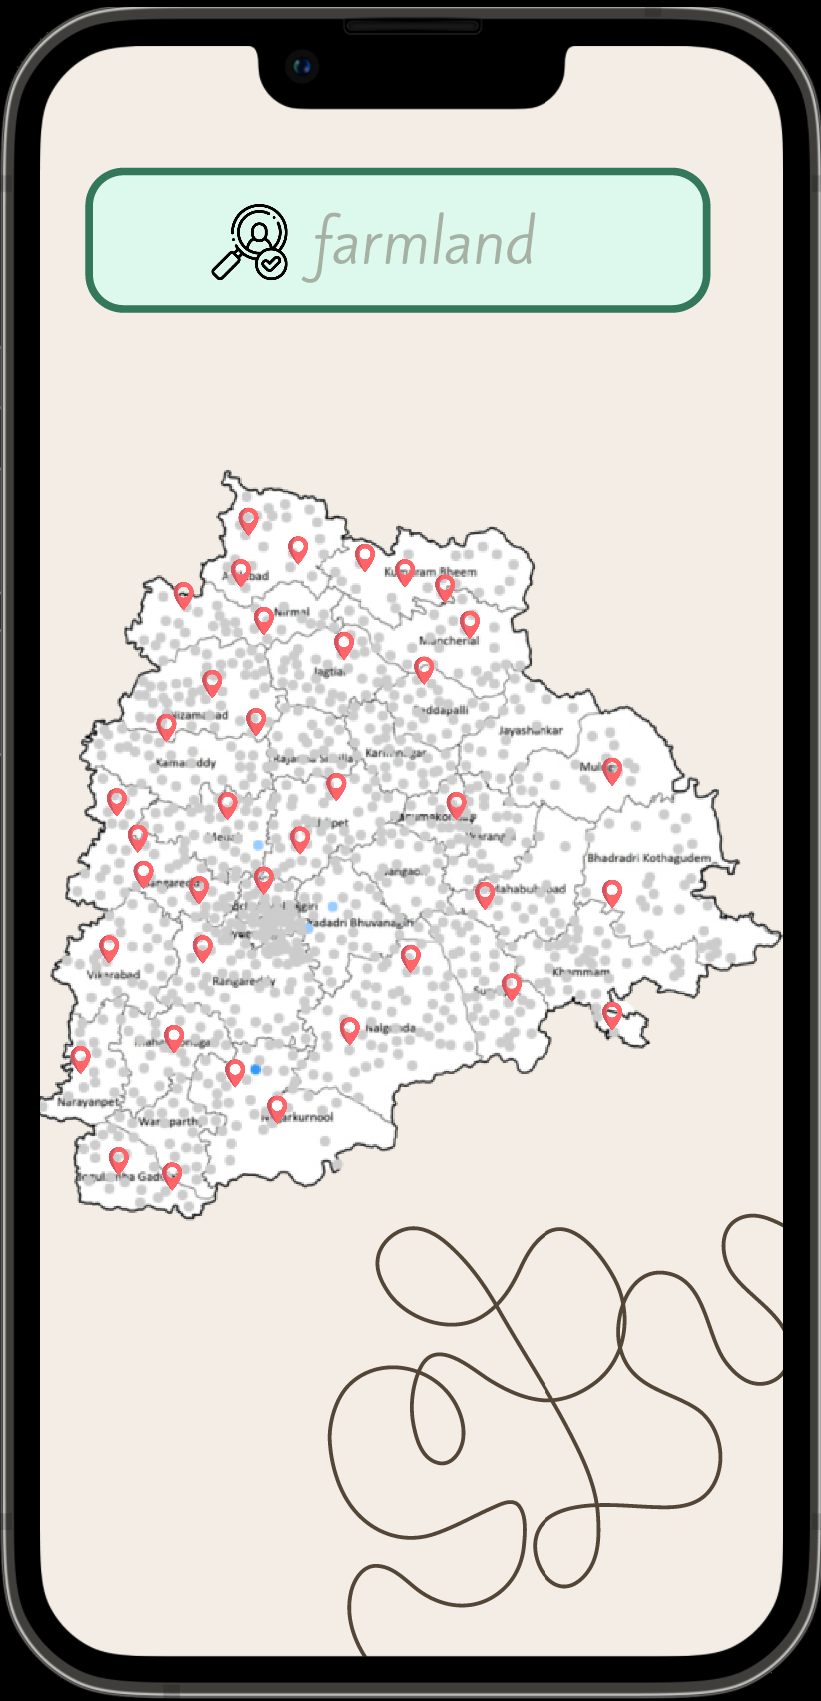
\includegraphics[width=0.4\textwidth,keepaspectratio]{figures/policyMakerMainPage.png}}
  \hfill

  \caption{Mockup}
\end{figure}

    \subsubsection{Hardware Interfaces}
    In this system, farmers need to have a smartphone with GPS or a desktop computer that they can, register and add their land to the application and track the changes and also their suggestions. Also, their smartphone should contain a touch screen or keyboard which helps them to start a discussion in the application, ask their questions and share their experiences. The policymaker should also have a smartphone or a desktop computer that login into their account and observe the farmer’s progress in the system. As we just have a mobile application for this program yet, they just need a smartphone.
    \subsubsection{Software Interfaces}
    Our system contains the following interfaces:\\
    Telangana’s map, We’ll use some API that allows us to
\begin{itemize}
    \item Locate the farmlands
    \item Getting information from water irrigation systems
    \item Getting data related to each land from sensors
    \item Getting meteorological information from Telangana’s government
\end{itemize}
The application should receive information about each land and update the data of each profile in real-time.\\
Also, we need push notification services when:
\begin{itemize}
    \item some urgent information change in the servers 
    \item they receive a message from policymakers
    \item someone sends a message in the discussion that they start or join.
\end{itemize}.

    \subsubsection{Communication Interfaces}
    The devices connect to DREAM via an internet connection.
\clearpage
\subsection{Functional Requirements}
    \subsubsection{List of Requirements}
    \begin{longtable}{ !\Vline c !\Vline p{0.9\linewidth} !\Vline}
    \hline
    \textbf{R1} & Farmers certified with an authentication\\
    \textbf{R2} & Policy-Makers certified with an authentication\\
    \textbf{R3} & Policy-Makers should register to the application with extra mandatory fields\\
    \textbf{R4} & Only Policy-Makers can observe all the farm land\\
    \textbf{R5} & Only Policy-Makers can best and worst farmers\\
    \textbf{R6} & Policy-Makers can choose farmers who received special incentives\\
    \textbf{R7} & Policy-Makers must identify those farmers who need to be helped\\
    \textbf{R8} & Farmers can be asked to provide useful best practices to the others\\
    \textbf{R9} & Farmers must accept the GPS location for the application\\
    \textbf{R10} & Farmers must insert their product to the system\\
    \textbf{R11} & Farmers can visualize data relevant to them\\
    \textbf{R12} & Farmers must insert the fertilizers that they are using to the system\\
    \textbf{R13} & Farmers could see the list of forecast related to their location\\
    \textbf{R14} & Farmers can insert any problem they face \\
    \textbf{R15} & Farmers can start a discussion \\
    \textbf{R16} & Farmers can request for help and suggestions by other farmers \\
    \textbf{R17} & Farmers can join to an existing discussion \\
    \textbf{R18} & Farmers can terminate their own discussion \\
    \textbf{R19} & The system should receive the data related to meteorological short-term and long-term forecasts from Telengana's governments \\
    \textbf{R20} & The system should suggest fertilizer based on the farmers locations and products \\
    \textbf{R21} & The system should receive the data from sensors periodically \\
    \textbf{R22} & The system should receive data from water irrigation system periodically\\
    \textbf{R23} & The system should send notifications about the farm land to the farmers\\
    \textbf{R24} & The system sends a notification to farmers if they receive new message\\
    \textbf{R25} & The system sends a notification to farmers if the humidity if water decrease\\
    \textbf{R26} & The system sends a notification to farmers if policymakers choose them as worst or best farmers\\
    \hline
\end{longtable}

\clearpage
    \subsubsection{Mapping}
    \arrayrulecolor{tableBorderColor}
\setlength\arrayrulewidth{1pt}
\rowcolors{2}{white}{tableHighlightColor}
\setlength\LTleft{0pt}
\begin{longtable}{ !\Vline c !\Vline p{0.3\linewidth} !\Vline p{0.6\linewidth} !\Vline}
    \hline
    \multicolumn{1}{|c|}{\textbf{Goal}} & \multicolumn{1}{c|}{\textbf{Domain assumption}} & \multicolumn{1}{c|}{\textbf{Requirements}}\\
    G1 & D1,D4,D5,D13 & R1,R9,R10, R12,R13,R19,R21,R22\\
    G2 & D4,D5 & R2,R3,R4, R10,R21,R22\\
    G3 & D1,D4,D5,D7,D8,D10 & R2,R3,R4,R6,R10,R21,R22,R26\\
    G4 & D1,D4,D5,D7,D8 & R2,R3,R4,R7,R10,R21,R22,R26\\
    
    G5 & D1,D2,D11 & R1,R15,R16,R17, R24\\
    G6 & D1,D2,D11 & R1,R17, R18\\
    G7 & D1,D9,D11,D13 & R1,R15,R17,R24\\
    G8 & D1, D9 & R1,R15,R17,R18\\
    G9 & D1,D2,D11 & R1,R16,R18\\
    G10 & D9,D11 & R1,R14\\
    G11 & D1,D9,D11,D13 & R1,R9,R17,R18, R24\\
    G12 & D1,D4,D13 & R8, R10,R23,R25\\
    
    \hline
\end{longtable}

\arrayrulecolor{tableBorderColor}
\setlength\arrayrulewidth{1pt}
\rowcolors{2}{white}{white}
\setlength\LTleft{0pt}
\begin{longtable}{ !\Vline c !\Vline p{0.9\linewidth} !\Vline}
    \hline
    \cellcolor{tableHighlightColor} \textbf{G1} & Allow farmers to see the details of their farm lands\\ \hline
     \cellcolor{purpleHiglight} \textbf{D1} & every farmer has at least one land\\ \hline
       \cellcolor{purpleHiglight} \textbf{D4} & farmers insert all of the information about production correctly\\ \hline
        \cellcolor{purpleHiglight} \textbf{D5} & farmer insert all of the information correctly\\ \hline
          \cellcolor{purpleHiglight} \textbf{D13} &  each user has a smartphone \\ \hline
    \cellcolor{pinkHighlight} \textbf{R1} & Farmers certified with an authentication\\
    \hline
    \cellcolor{pinkHighlight} \textbf{R9} & Farmers must accept the GPS location for the application\\
    \hline
    \cellcolor{pinkHighlight} \textbf{R10} & Farmers must insert their product to the system\\
    \hline
    \cellcolor{pinkHighlight} \textbf{R12} & Farmers must insert the fertilizers that they are using to the system\\
    \hline
    \cellcolor{pinkHighlight} \textbf{R13} & Farmers could see the list of forecast related to their location\\
    \hline
    \cellcolor{pinkHighlight} \textbf{R19} & The system should receive the data related to meteorological short-term and long-term forecasts from Telengana's governments\\
    \hline
    \cellcolor{pinkHighlight} \textbf{R21} & The system should suggest fertilizer based on the farmers locations and products\\
    \hline
    \cellcolor{pinkHighlight} \textbf{R22} & The system should receive data from water irrigation system periodically\\
    \hline
    \cellcolor{tableHighlightColor} \textbf{G2} & Allow policy makers to see the details of different lands\\ \hline
       \cellcolor{purpleHiglight} \textbf{D4} & farmers insert all of the information about production correctly\\ \hline
        \cellcolor{purpleHiglight} \textbf{D5} & farmer insert all of the information correctly\\ 
        \hline
    \cellcolor{pinkHighlight} \textbf{R2} & Policy-Makers certified with an authentication\\
    \hline
    \cellcolor{pinkHighlight} \textbf{R3} & Policy-Makers should register to the application with extra mandatory fields\\
    \hline
    \cellcolor{pinkHighlight} \textbf{R4} & Only Policy-Makers can observe all the farm land\\
    \hline
    \cellcolor{pinkHighlight} \textbf{R10} & Farmers must insert their product to the system\\
    \hline
    \cellcolor{pinkHighlight} \textbf{R21} & The system should receive the data from sensors periodically\\
    \hline
    \cellcolor{pinkHighlight} \textbf{R22} & The system should receive data from water irrigation system periodically\\
    \hline
    \cellcolor{tableHighlightColor} \textbf{G3} & Allow policy makers to identify farmers who are performing well\\ \hline
     \cellcolor{purpleHiglight} \textbf{D1} & every farmer has at least one land\\ \hline
       \cellcolor{purpleHiglight} \textbf{D4} & farmers insert all of the information about production correctly\\ \hline
        \cellcolor{purpleHiglight} \textbf{D5} & farmer insert all of the information correctly\\ \hline
          \cellcolor{purpleHiglight} \textbf{D7} &  amount of used water report correctly by irrigation system \\ \hline
          \cellcolor{purpleHiglight} \textbf{D8} &  policy maker asses the former based on true information \\ \hline
          \cellcolor{purpleHiglight} \textbf{D10} &  amount of reported humidity is correctly \\ \hline
    \cellcolor{pinkHighlight} \textbf{R2} & Policy-Makers certified with an authentication\\
    \hline
    \cellcolor{pinkHighlight} \textbf{R3} & Policy-Makers should register to the application with extra mandatory fields\\
    \hline
    \cellcolor{pinkHighlight} \textbf{R4} & Only Policy-Makers can observe all the farm land\\
    \hline
    \cellcolor{pinkHighlight} \textbf{R6} & policy-Makers can choose farmers who received special incentives\\
    \hline
    \cellcolor{pinkHighlight} \textbf{R10} & Farmers must insert their product to the system\\
    \hline
    \cellcolor{pinkHighlight} \textbf{R21} & The system should receive the data from sensors periodically\\
    \hline
    \cellcolor{pinkHighlight} \textbf{R22} & The system should receive data from water irrigation system periodically\\
    \hline
    \cellcolor{pinkHighlight} \textbf{R26} & The system sends a notification to farmers if policymakers choose them as worst or best farmers\\
    \hline
    \cellcolor{tableHighlightColor} \textbf{G4} & Allow policy makers to identify farmers who need help\\ \hline
    \cellcolor{purpleHiglight} \textbf{D1} & every farmer has at least one land\\ \hline
       \cellcolor{purpleHiglight} \textbf{D4} & farmers insert all of the information about production correctly\\ \hline
        \cellcolor{purpleHiglight} \textbf{D5} & farmer insert all of the information correctly\\ \hline
          \cellcolor{purpleHiglight} \textbf{D7} &  amount of used water report correctly by irrigation system \\ \hline
          \cellcolor{purpleHiglight} \textbf{D8} &  policy maker asses the former based on true information \\ \hline
    \cellcolor{pinkHighlight} \textbf{R2} & Policy-Makers certified with an authentication\\
    \hline
    \cellcolor{pinkHighlight} \textbf{R3} & Policy-Makers should register to the application with extra mandatory fields\\
    \hline
    \cellcolor{pinkHighlight} \textbf{R4} & Only Policy-Makers can observe all the farm land\\
    \hline
    \cellcolor{pinkHighlight} \textbf{R7} & Policy-Makers must identify those farmers who need to be helped\\
    \hline
    \cellcolor{pinkHighlight} \textbf{R10} & Farmers must insert their product to the system\\
    \hline
    \cellcolor{pinkHighlight} \textbf{R21} & The system should receive the data from sensors periodically\\
    \hline
    \cellcolor{pinkHighlight} \textbf{R22} & The system should receive data from water irrigation system periodically\\
    \hline
    \cellcolor{pinkHighlight} \textbf{R26} & The system sends a notification to farmers if policymakers choose them as worst or best farmers\\
    \hline
    \cellcolor{tableHighlightColor} \textbf{G5} & Allow farmers to create new forum\\ \hline
     \cellcolor{purpleHiglight} \textbf{D1} & The internet works properly\\ \hline
      \cellcolor{purpleHiglight} \textbf{D2} &  Its better for users to have smartphones\\ \hline
      \cellcolor{purpleHiglight} \textbf{D11} &  farmers insert problems about farm land,production\\ \hline
    \cellcolor{pinkHighlight} \textbf{R1} & Users certified with an authentication\\
    \hline
    \cellcolor{pinkHighlight} \textbf{R15} & Farmers can start a discussion\\
    \hline
    \cellcolor{pinkHighlight} \textbf{R16} & Farmers can request for help and suggestions by other farmers\\
    \hline
    \cellcolor{pinkHighlight} \textbf{R17} & Farmers can join to an existing discussion\\
    \hline
    \cellcolor{pinkHighlight} \textbf{R24} & The system sends a notification to farmers if they receive new message\\
    \hline
    \cellcolor{tableHighlightColor} \textbf{G6} & Allow farmers to join in discussions\\ \hline
     \cellcolor{purpleHiglight} \textbf{D1} & The internet works properly\\ \hline
      \cellcolor{purpleHiglight} \textbf{D2} &  Its better for users to have smartphones\\ \hline
      \cellcolor{purpleHiglight} \textbf{D11} &  farmers insert problems about farm land,production\\ \hline
      \cellcolor{pinkHighlight} \textbf{R1} & Farmers certified with an authentication\\
    \hline
    \cellcolor{pinkHighlight} \textbf{R17} & Farmers can join to an existing discussion\\
    \hline
    \cellcolor{pinkHighlight} \textbf{R18} &  Farmers can terminate their own discussion\\
    \hline
    \cellcolor{tableHighlightColor} \textbf{G7} &  Allow farmers to send message in discussions\\ \hline
     \cellcolor{purpleHiglight} \textbf{D1} & The internet works properly\\ \hline
     \cellcolor{purpleHiglight} \textbf{D9} & just authenticated farmer can send message to forum\\ \hline
       \cellcolor{purpleHiglight} \textbf{D11} & farmers insert problems about farm land,production\\ \hline
       
      \cellcolor{purpleHiglight} \textbf{D13} &  each user has a smartphone\\ \hline
    \cellcolor{pinkHighlight} \textbf{R1} & Farmers certified with an authentication\\
    \hline
    \cellcolor{pinkHighlight} \textbf{R15} & Farmers can start a discussion\\
    \hline
    \cellcolor{pinkHighlight} \textbf{R17} & Farmers can join to an existing discussion\\
    \hline
    \cellcolor{pinkHighlight} \textbf{R24} & The system sends a notification to farmers if they receive new message\\
    \hline
    
    \cellcolor{tableHighlightColor} \textbf{G8} & Allow farmers to create new forum\\ \hline
    \cellcolor{purpleHiglight} \textbf{D1} & The internet works properly\\ \hline
     \cellcolor{purpleHiglight} \textbf{D9} & just authenticated farmer can send message to forum\\ \hline
    \cellcolor{pinkHighlight} \textbf{R1} & Farmers certified with an authentication\\
    \hline
    \cellcolor{pinkHighlight} \textbf{R15} & Farmers can start a discussion\\
    \hline
    \cellcolor{pinkHighlight} \textbf{R17} & Farmers can join to an existing discussion\\
    \hline
    \cellcolor{pinkHighlight} \textbf{R18} &  Farmers can terminate their own discussion\\
    \hline
    \cellcolor{tableHighlightColor} \textbf{G9} & Allow farmers to leave in discussions\\ \hline
     \cellcolor{purpleHiglight} \textbf{D1} & The internet works properly\\ \hline
      \cellcolor{purpleHiglight} \textbf{D2} &  Its better for users to have smartphones\\ \hline
      \cellcolor{purpleHiglight} \textbf{D11} &  farmers insert problems about farm land,production\\ \hline
      \cellcolor{purpleHiglight} \textbf{D11} &  farmers insert problems about farm land,production\\ \hline
      \cellcolor{pinkHighlight} \textbf{R1} & Farmers certified with an authentication\\
    \hline
    \cellcolor{pinkHighlight} \textbf{R16} & Farmers can leave a discussion\\
    \hline
    \cellcolor{pinkHighlight} \textbf{R18} &  Farmers can terminate their own discussion\\
    \hline
    \cellcolor{tableHighlightColor} \textbf{G10} & Allow farmers to ask problems\\ \hline
      \cellcolor{purpleHiglight} \textbf{D9} & just authenticated farmer can send message to forum\\ \hline
      \cellcolor{purpleHiglight} \textbf{D11} & farmers insert problems about farm land,production\\ \hline
    \cellcolor{pinkHighlight} \textbf{R1} & Farmers certified with an authentication\\
    \hline
    \cellcolor{pinkHighlight} \textbf{R14} & Farmers can insert any problem they face \\
    \hline
    \cellcolor{tableHighlightColor} \textbf{G11} & Allow farmers to answer to problems\\ \hline
     \cellcolor{purpleHiglight} \textbf{D1} & The internet works properly\\ \hline
     \cellcolor{purpleHiglight} \textbf{D9} & just authenticated farmer can send message to forum\\ \hline
       \cellcolor{purpleHiglight} \textbf{D11} & farmers insert problems about farm land,production\\ \hline
      \cellcolor{purpleHiglight} \textbf{D13} &  each user has a smartphone\\ \hline
    \cellcolor{pinkHighlight} \textbf{R1} & Farmers certified with an authentication\\
    \hline
    \cellcolor{pinkHighlight} \textbf{R15} & Farmers can start a discussion\\
    \hline
    \cellcolor{pinkHighlight} \textbf{R17} & Farmers can join to an existing discussion\\
    \hline
    \cellcolor{pinkHighlight} \textbf{R18} &  Farmers can terminate their own discussion\\
    \hline
    \cellcolor{pinkHighlight} \textbf{R24} & The system sends a notification to farmers if they receive new message\\ \hline
    \cellcolor{tableHighlightColor} \textbf{G12} & Show farmers some personal suggestion\\ \hline
     \cellcolor{purpleHiglight} \textbf{D1} & every farmer has at least one land\\ \hline
      \cellcolor{purpleHiglight} \textbf{D4} & farmers insert all of the information about production correctly\\ \hline
      \cellcolor{purpleHiglight} \textbf{D13} & each user has a smartphone\\ \hline
    \cellcolor{pinkHighlight} \textbf{R8} & Farmers can be asked to provide useful best practices to the others\\
    \hline
    \cellcolor{pinkHighlight} \textbf{R10} & Farmers must insert their product to the system\\
    \hline
    \cellcolor{pinkHighlight} \textbf{R23} & The system should send notifications about the farm land to the farmers\\
    \hline
    \cellcolor{pinkHighlight} \textbf{R25} & The system sends a notification to farmers if the humidity if water decrease\\
    \hline
    
\end{longtable}
    \subsubsection{Use Cases}
    \paragraph{Use Cases Description}
    
\begin{table}[H]
%\centering
\begin{tabular}{|l|l|}
\hline
\normalsize	
\textbf{Name} & Sign up\\\hline
\textbf{Actor} & farmer\\\hline
\textbf{Entry conditions} & Use the user has installed the application on her/his device\\\hline
\textbf{Event flow}  &  1. Click on "Sign Up" button"\\ 
&2. Fill all the mandatory fields and provide the necessary information\\
&3. Click on "Confirm" button\\
&4.the system saves the data \\\hline
\textbf{Exit conditions} & The user successfully registered and now he's able to use the application. \\\hline
\textbf{Exceptions }& 
1.the user is already signed up \\&
2.the user didn't fill all of the mandatory fields with valid data\\&
3.The username is already taken\\&
4.the e-mail is already registered\\&
5.All the exception are handled by notifying the user and taking\\& him back to the sign up activity
\\\hline
\end{tabular}
%\caption{\label{tab:widgets}An example table.}
\end{table}




\begin{table}[H]
%\centering
\begin{tabular}{|l|l|}
\hline
\normalsize	
\textbf{Name} & log in\\\hline
\textbf{Actor} & farmer\\\hline
\textbf{Entry conditions} & The user is previously successfully signed up 
\\&and has the application installed in his/her device\\\hline
\textbf{Event flow}  &  1. The user opens the application on his/device\\&
2. He enters his credentials in the “Username” and “Password” fields of\\&
the home page of “DREAM”\\&
3. The user clicks on the “Log in” button\\&
4. The user is successfully logged in his/her “DREAM”\\&
the system automatically redirects him/her to the home page\\\hline
\textbf{Exit conditions} & The user is successfully redirected to the home page \\\hline
\textbf{Exceptions }& 
1. The user enters an invalid Username\\&
2. The user enters invalid Password\\&
3. All the exceptions are handled by notifying the user and taking\\&
him/her back to the login activity\\&
\\\hline
\end{tabular}
%\caption{\label{tab:widgets}An example table.}
\end{table}


\begin{table}[H]
%\centering
\begin{tabular}{|l|l|}
\hline
\normalsize	
\textbf{Name} & insert the initial information \\\hline
\textbf{Actor} & farmer\\\hline
\textbf{Entry conditions}& The user has already logged in\\\hline
\textbf{Event flow} &1. The farmer select the farm land location\\&
2. He enters his credentials in the “Username” ,“land name” ,"email"\\& 
,"product","amount"and"fertilizer"\\&
3. the user click on  the register button\\&
4. The user is successfully logged in his/her “DREAM”\\&
the system automatically redirects him/her to the home page\\\hline
\textbf{Exit conditions} & The user is successfully redirected to the home page \\\hline
\textbf{Exceptions }& 
1. The user enters an empty Username field\\&
2. The user enters an empty land name field\\&
3. The user enters an empty Email field\\&
4. the user enter empty product \& amount field\\\hline
\end{tabular}
%\caption{\label{tab:widgets}An example table.}
\end{table}




\begin{table}[H]
%\centering
\begin{tabular}{|l|l|}
\hline
\normalsize	
\textbf{Name} & analyse  the initial conditions\\\hline
\textbf{Actor} & farmer\\\hline
\textbf{Entry conditions} & The farmer insert completely initial information and report \\\hline
\textbf{Event flow}  &  1.The system get initial information\\&
2. It get weather forecast based on GPS and land location \\&
3. system analyze the information \\\hline
\textbf{Exit conditions} & make personalized suggestion \\\hline
\textbf{Exceptions }& 
1. the forecast data is not accurate or invalid \\&
2. input data has conflict\\&
3. All the exceptions are handled by notifying the user and taking\\&
him/her back to the insert information page\\&
\\\hline
\end{tabular}
%\caption{\label{tab:widgets}An example table.}
\end{table}


\begin{table}[H]
%\centering
\begin{tabular}{|l|l|}
\hline
\normalsize	
\textbf{Name} & make personalized suggestion\\\hline
\textbf{Actor} & farmer\\\hline
\textbf{Entry conditions} & analysing of initial information has completed\\\hline
\textbf{Event flow}  &  1. get the analysing of initial information \\ 
&2. apply the ML/AL algorithm find best crop and fertilizer\\
&3. show the result to farmer \\
\textbf{Exit conditions} & The user successfully registered and now he's able to use the application. \\\hline
\textbf{Exceptions }& 
1.the user is already signed up \\&
2.the user didn't fill all of the mandatory fields with valid data\\&
3.The username is already taken\\&
4.the e-mail is already registered\\&
5.All the exception are handled by notifying the user and taking\\& him back to the sign up activity
\\\hline
\end{tabular}
%\caption{\label{tab:widgets}An example table.}
\end{table}

\begin{table}[H]
%\centering
\begin{tabular}{|l|l|}
\hline
\normalsize	
\textbf{Name} & Measure used water\\\hline
\textbf{Actor} & Irrigation system\\\hline
\textbf{Entry conditions} & Install irrigation system on the land\\\hline
\textbf{Event flow}  &  1.The irrigation system measure used water in specific frequency-time\\\hline
\textbf{Exit conditions} & Send measured data to access point \\\hline
\textbf{Exceptions}& 
1. Measured used water is not possible \\&
2. Irrigation system doesn't work correctly\\&
3. All the exceptions are handled by sent notification to access point 
\\\hline
\end{tabular}
%\caption{\label{tab:widgets}An example table.}
\end{table}


\begin{table}[H]
%\centering
\begin{tabular}{|l|l|}
\hline
\normalsize	
\textbf{Name} & Measure soil humidity\\\hline
\textbf{Actor} & Sensor\\\hline
\textbf{Entry conditions} & Install sensor with the specific distance in depth of soil\\\hline
\textbf{Event flow} & 1.the installed sensors sense humidity \\\hline
\textbf{Exit conditions} & Send measured data to access point \\\hline
\textbf{Exceptions}& 
1. Measured used soil humidity is not possible \\&
2. Sensors doesn't work correctly\\&
3. All the exceptions are handled by sent notification to access point 
\\\hline
\end{tabular}
%\caption{\label{tab:widgets}An example table.}
\end{table}



\begin{table}[H]
%\centering
\begin{tabular}{|l|l|}
\hline
\normalsize	
\textbf{Name} & send collected data to the  access point\\\hline
\textbf{Actor} & system\\\hline
\textbf{Entry conditions} & measure soil humidity  OR  measure used water OR  report forecast weather \\\hline
\textbf{Event flow}  &  1. get the measured soil humidity from sensors\\&
OR get measured used water from irrigation system \\&
OR get weather forecast from meteorological station \\&
2. collect information and prepare it to analyse\\\hline
\textbf{Exit conditions} & analyse the collected info \\\hline
\textbf{Exceptions }& 
1.The network doesn't work correctly  \\&
2.Sensors doesn't work correctly \\&
3.Irrigation systems doesn't work correctly \\&
4.Weather forecast doesn't report information correctly\\&
5.All the exceptions are handled by sent notification to access point
\\\hline
\end{tabular}
%\caption{\label{tab:widgets}An example table.}
\end{table}



\begin{table}[H]
%\centering
\begin{tabular}{|l|l|}
\hline
\normalsize	
\textbf{Name} & report forecast weather t\\\hline
\textbf{Actor} & Meteorological station\\\hline
\textbf{Entry conditions} & Meteorological station connects to the internet and GPS \\\hline
\textbf{Event flow} & 1.connect to the meteorological satellite \\&
2. get the weather forecast\\&
3.get the location information by GPS\\\hline
\textbf{Exit conditions} & send collected data to the access point \\\hline
\textbf{Exceptions }& 
1.The network doesn't work correctly  \\&
2.GPS doesn't work correctly \\&
3. Meteorological station devices work correctly\\&
5.All the exceptions are handled by sent notification to access point
\\\hline
\end{tabular}
%\caption{\label{tab:widgets}An example table.}
\end{table}

\begin{table}[H]
%\centering
\begin{tabular}{|l|l|}
\hline
\normalsize	
\textbf{Name} & evaluate farmer performance\\\hline
\textbf{Actor} & policy maker\\\hline
\textbf{Entry conditions} & analyse the collected info   \\\hline
\textbf{Event flow} & 1.get analysing collected environment data \\&
2. identify good and bad farmer based on analysed data\\\hline
\textbf{Exit conditions} & after identifying the high and  low performance farmer  \\\hline
\textbf{Exceptions }& 
1.analysed data is not accrued\\&
2.analysed data  has a shortage information \\&
3.analysed data is not reliable and semantic meaning  \\&
5.All the exceptions are handled by sent notification to access point
\\\hline
\end{tabular}
%\caption{\label{tab:widgets}An example table.}
\end{table}

\begin{table}[H]
%\centering
\begin{tabular}{|l|l|}
\hline
\normalsize	
\textbf{Name} & visualize the analysed information \\\hline
\textbf{Actor} & farmer\\\hline
\textbf{Entry conditions} &  analyse the collected info  \\\hline
\textbf{Event flow} & 1.get analysed data \\&
2. apply the specific algorithm to visualized the data\\&
\\\hline
\textbf{Exit conditions} & result is ready to show to farmer  \\\hline
\textbf{Exceptions }& 
1. analyzed data doesn't have enough quality to analyzed that can be visualized \\&
2.data doesn't have semantic meaning 
\\\hline
\end{tabular}
%\caption{\label{tab:widgets}An example table.}
\end{table}

\paragraph{Use Cases Diagram}

\begin{figure}[H]
%\centering
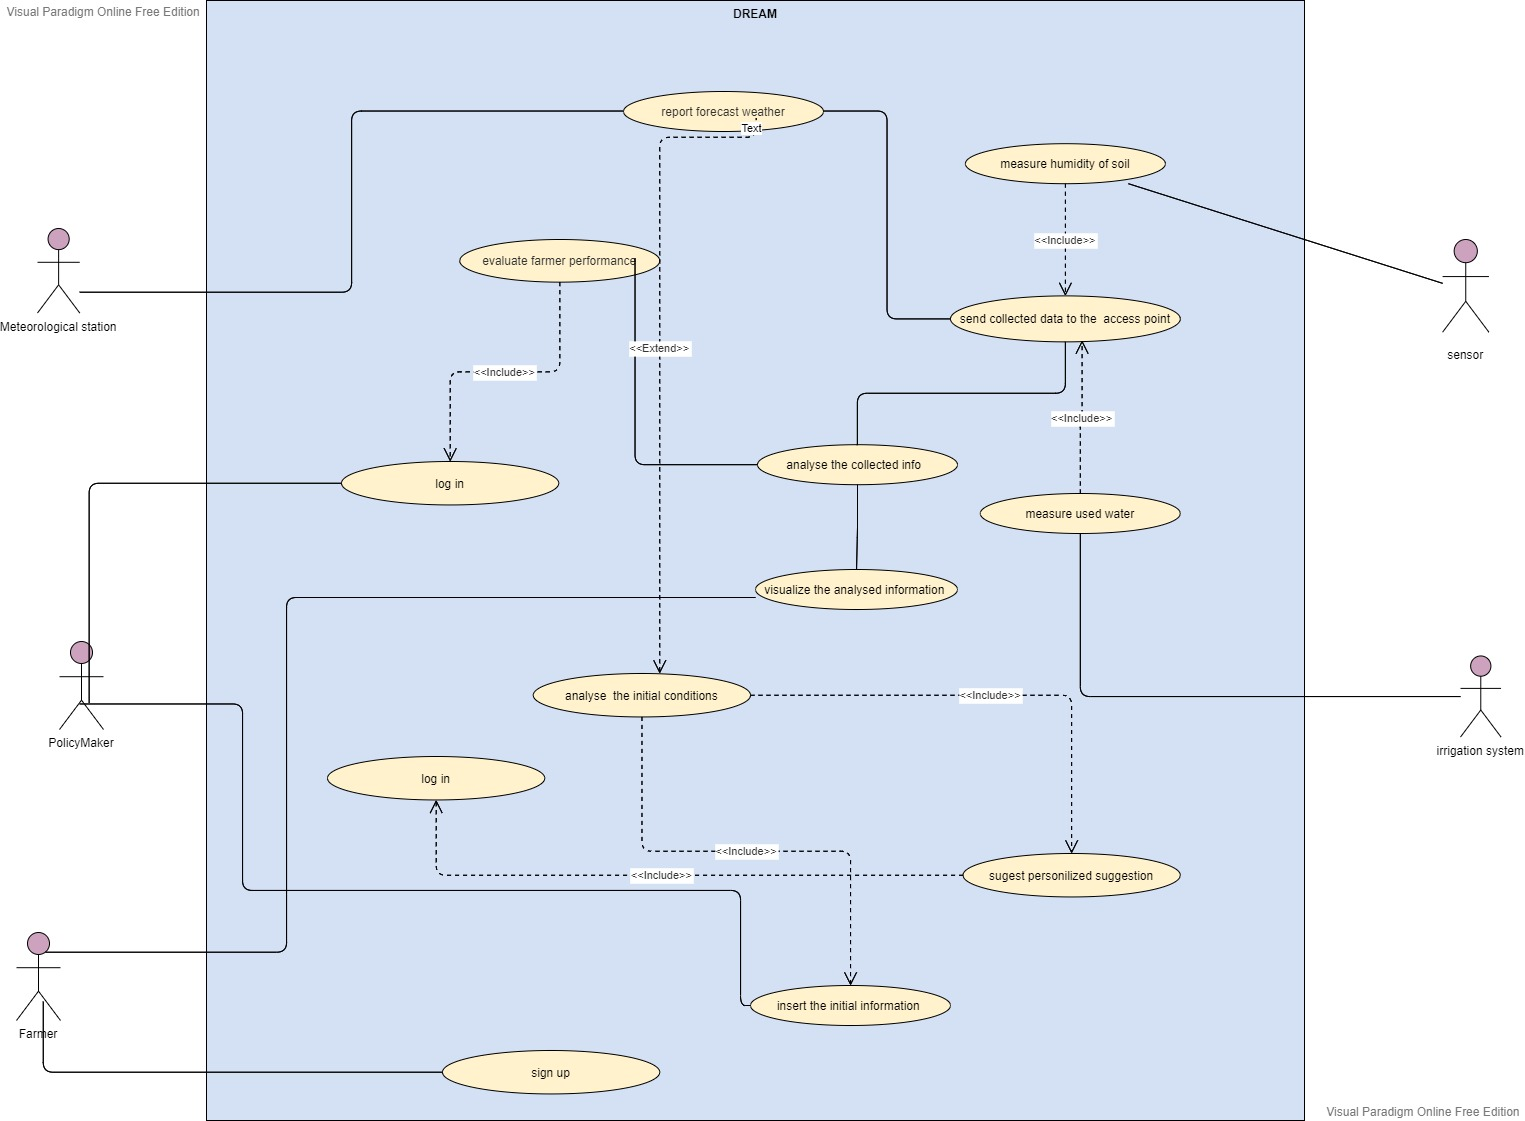
\includegraphics[width=1\textwidth]{figures/usecase.jpg}
%\caption{\label{fig:student } State Diagram 3 - evaluate the farmer by policymaker }
\end{figure}
       \subsubsection{Sequence diagram}
    \begin{figure}[H]
%\centering
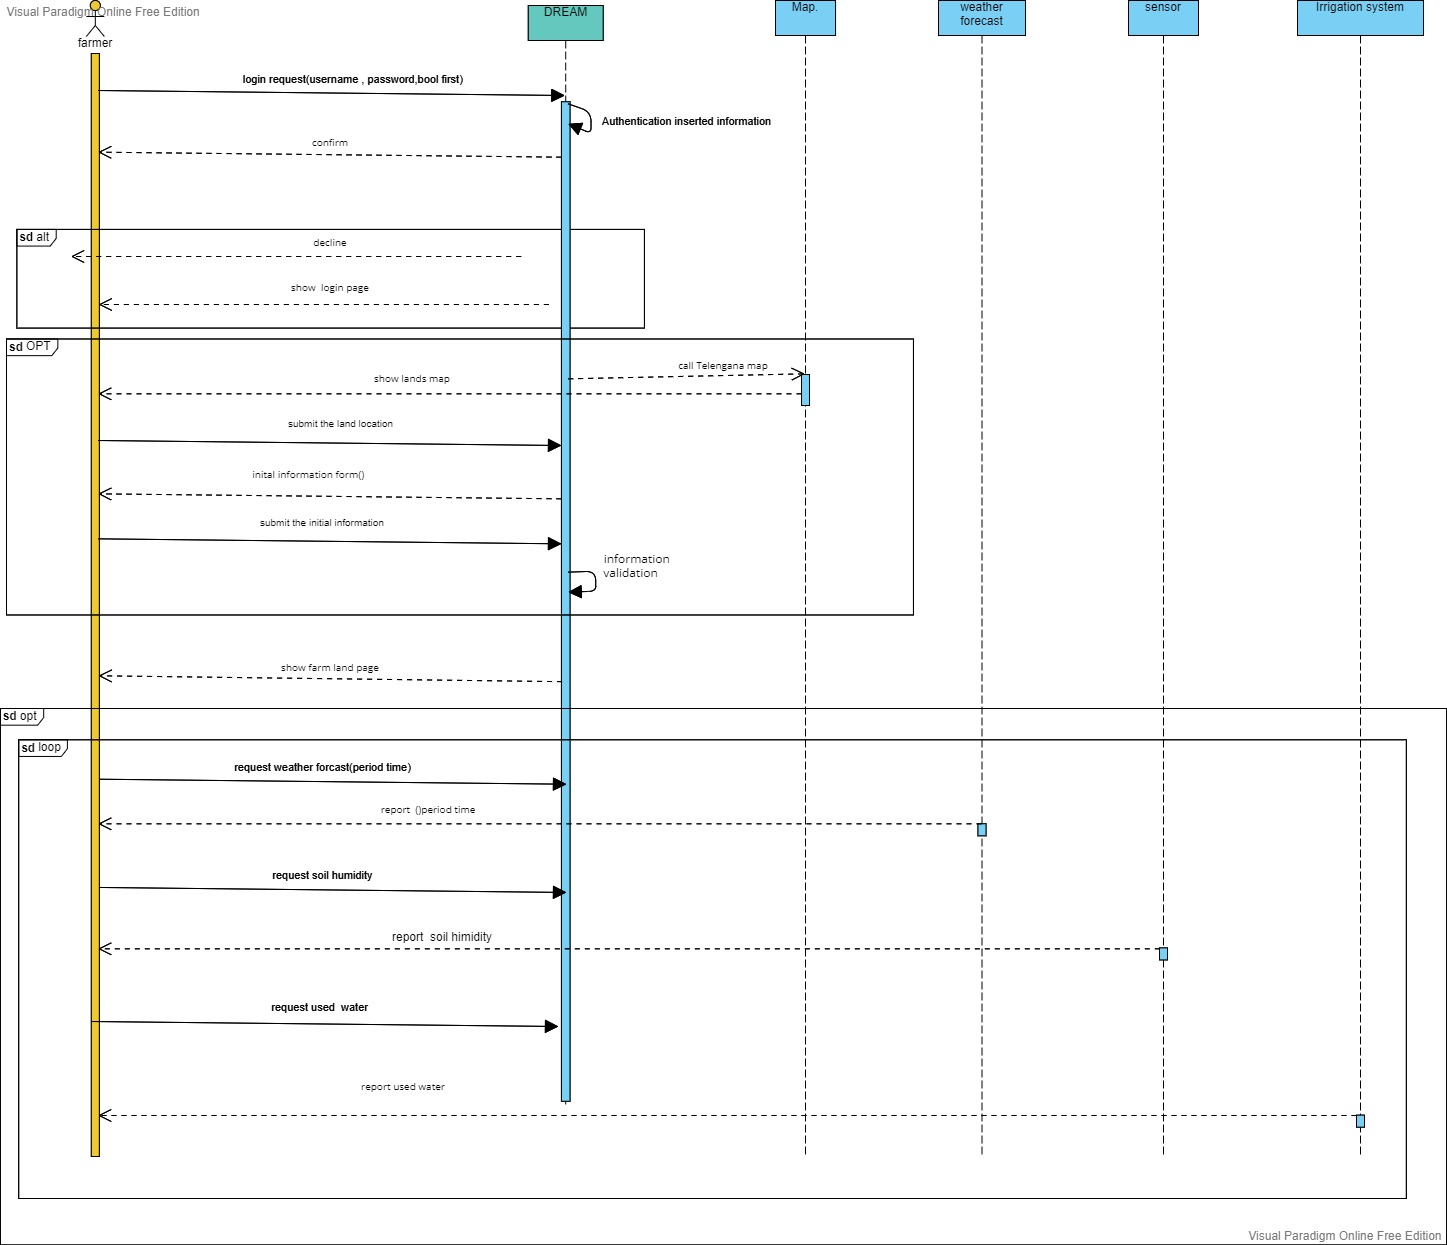
\includegraphics[width=1\textwidth]{figures/firstSequenceDiagram.jpg}
%\caption{\label{fig:student } State Diagram 3 - evaluate the farmer by policymaker }
\end{figure}
\begin{figure}[H]
%\centering
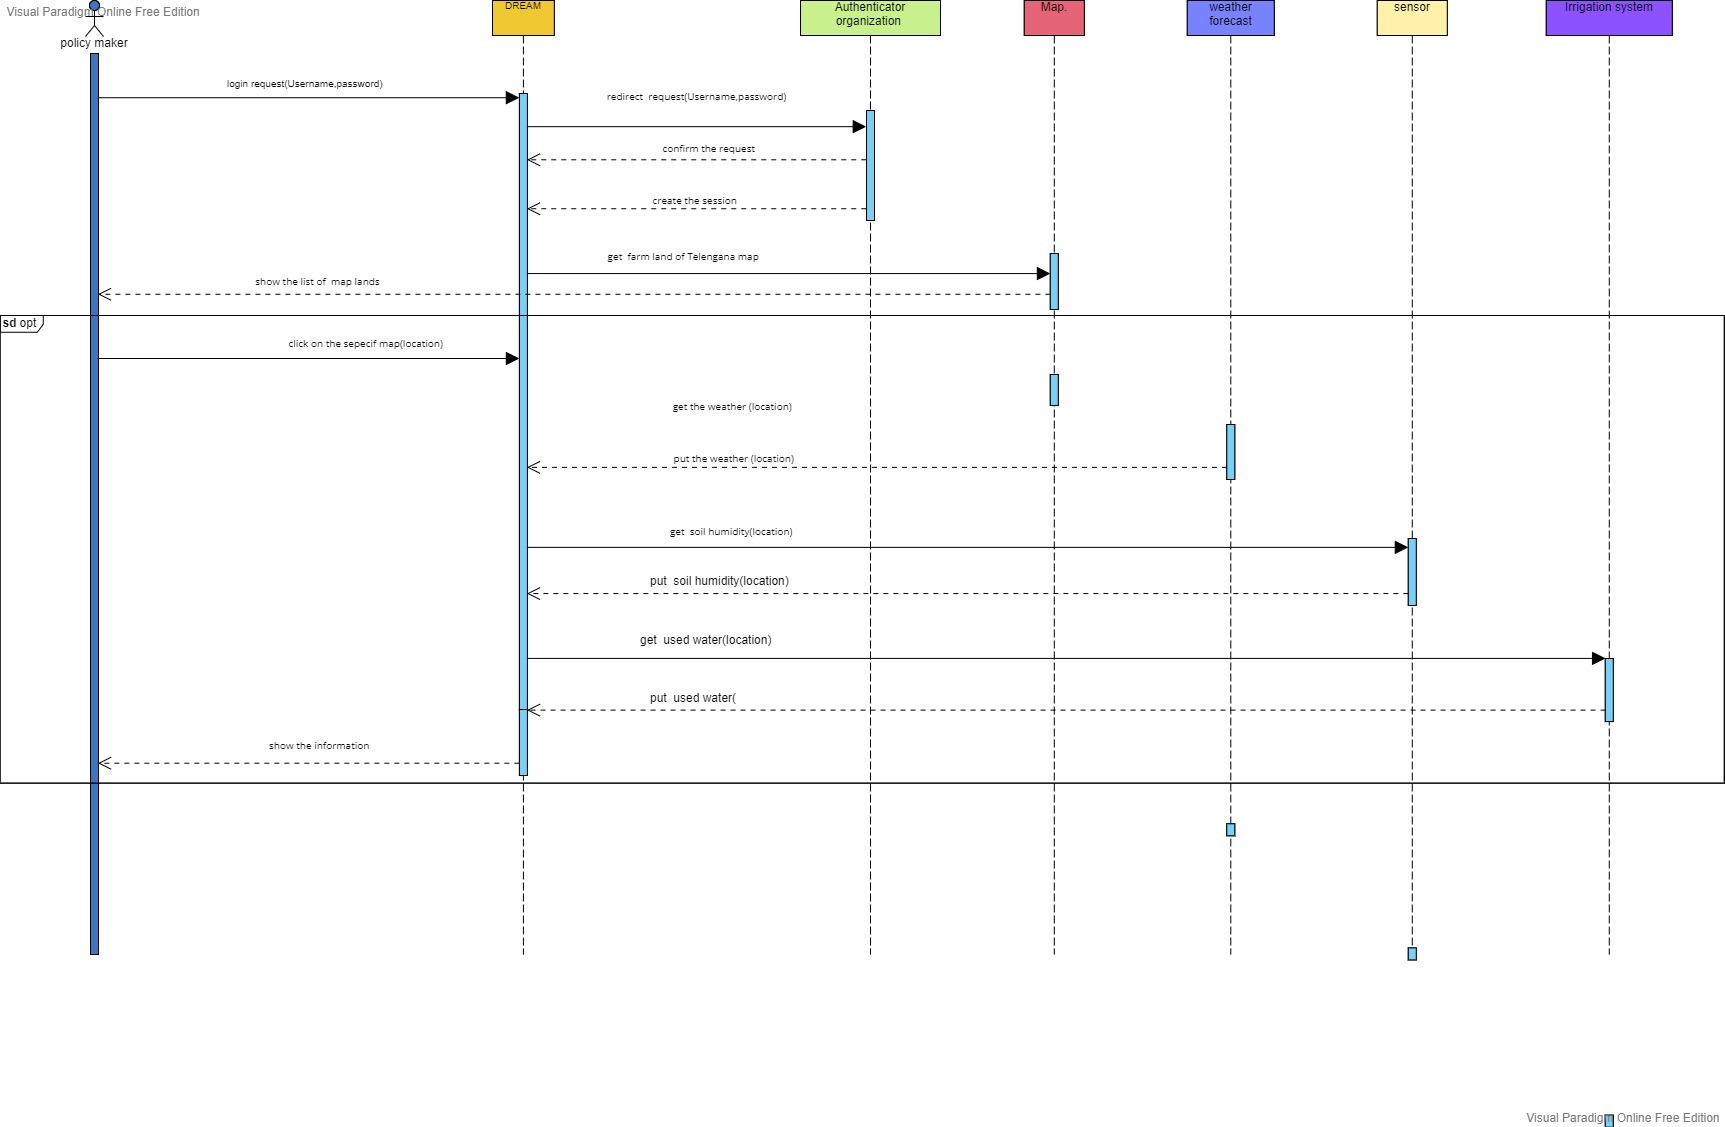
\includegraphics[width=1\textwidth]{figures/SecondSequenceDiagram.jpg}
%\caption{\label{fig:student } State Diagram 3 - evaluate the farmer by policymaker }
\end{figure}
\begin{figure}[H]
%\centering
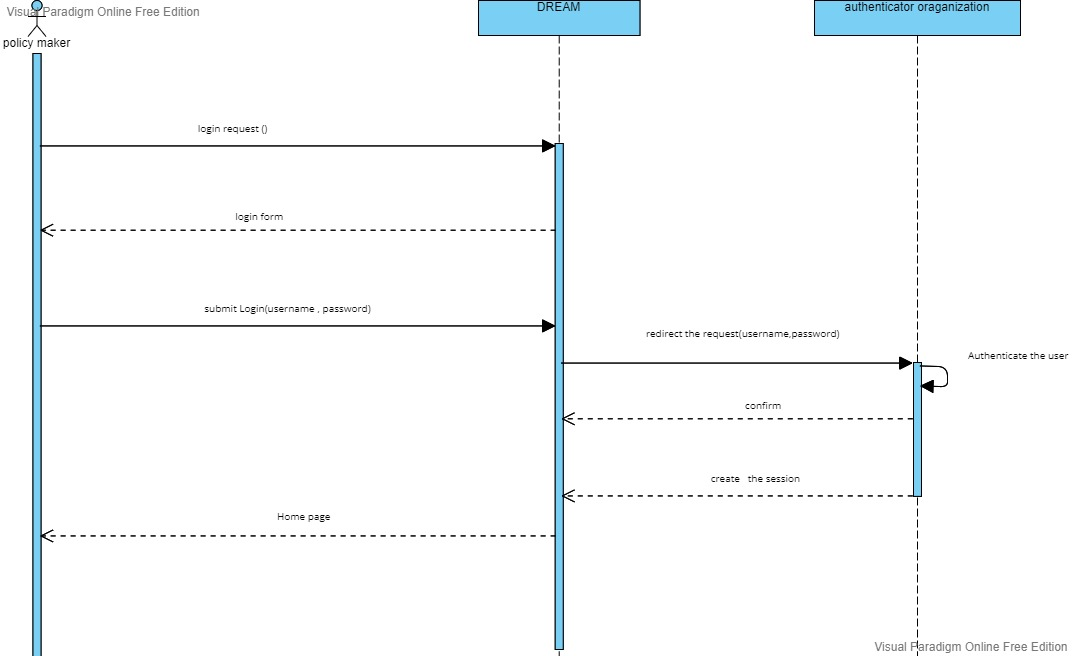
\includegraphics[width=1\textwidth]{figures/thirdSequenceDiagram.jpg}
%\caption{\label{fig:student } State Diagram 3 - evaluate the farmer by policymaker }
\end{figure}
\begin{figure}[H]
%\centering
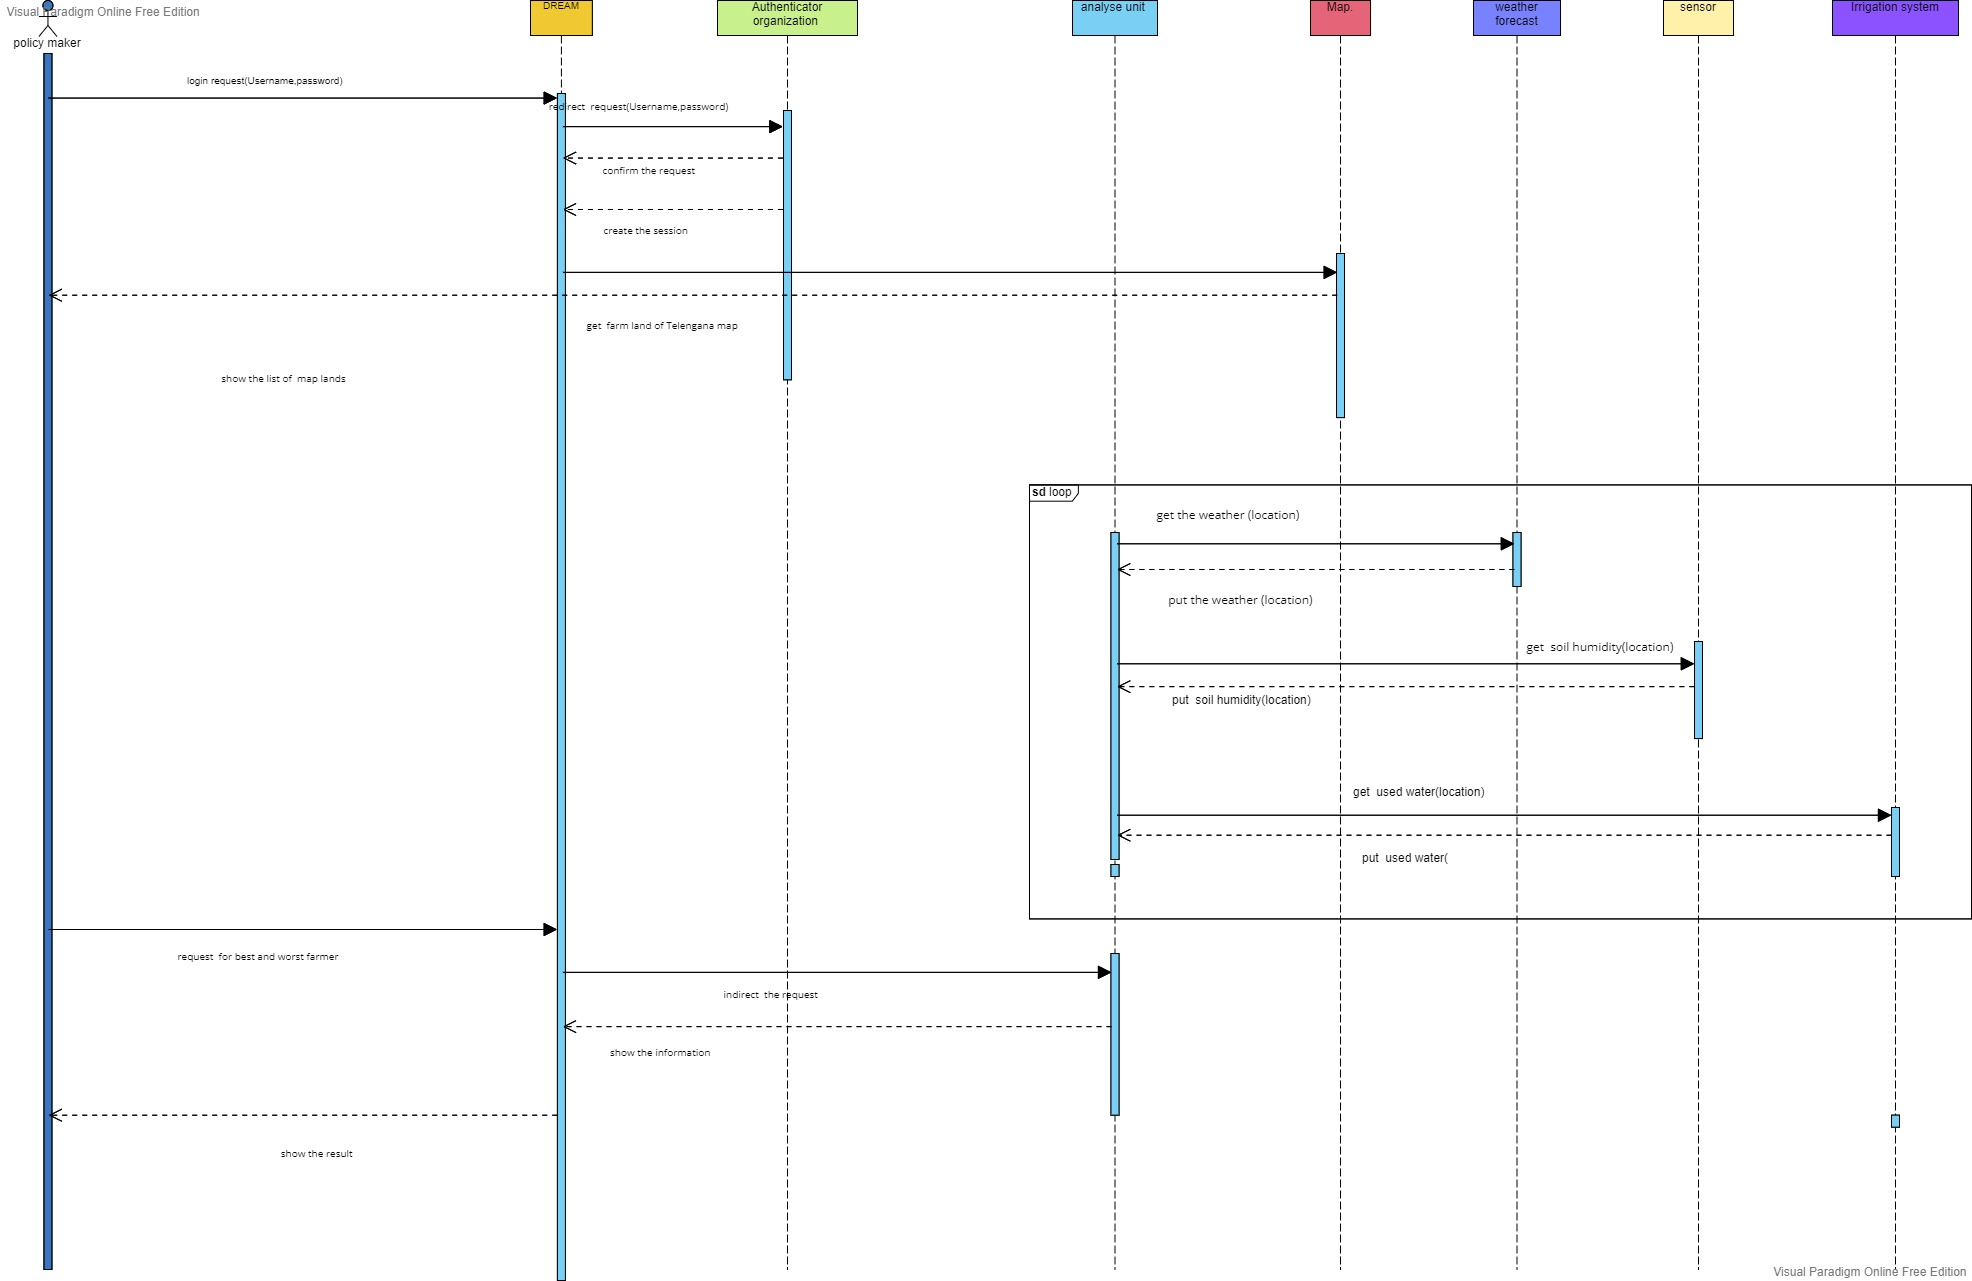
\includegraphics[width=1\textwidth]{figures/forthSequenceDiagram.jpg}
%\caption{\label{fig:student } State Diagram 3 - evaluate the farmer by policymaker }
\end{figure}

\begin{figure}[H]
%\centering
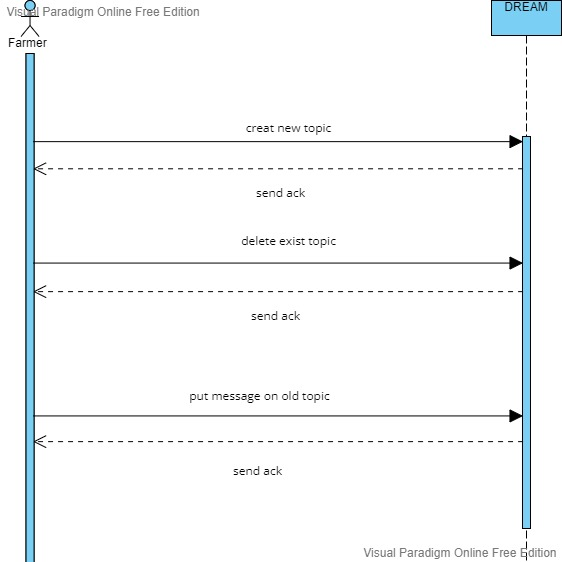
\includegraphics[width=1\textwidth]{figures/fifthSequenceDiagram.jpg}
%\caption{\label{fig:student } State Diagram 3 - evaluate the farmer by policymaker }
\end{figure}
    \subsubsection{Scenarios}
    
    Nila is going to plant potatoes on her farm and she wants to know which crop is compatible with the land situation, she enters her land location, used fertilizer and crop information finally system by checking the weather, make a decision that  potato is proportionate with entered data or not, and make a personalized suggestion to have the best result.
\newline
\newline
Aadhya is the framer that the quality crops is Less than the system predicted because its products were attacked by an unknown pest so she decides to ask her problem in the forum from other farmers to use their experience. first, check the FQA to find the answer, then if she doesn't find an appropriate answer create a new topic and wait for another one to answer her problem. Aarna is another farmer in our system that had the same problems login in DREAM and in the forum in the problem section after the see the problem answer it 
\newline
\newline



Krishna is a farmer who has been engaged in traditional farming for many years he wants to 
mechanize his farming methods, first install sensors and irrigation system to measure the humidity and use water then  He must sign up in the system. To do this, he first enters his basic information, including his user ID, land name, product, and fertilizer used in the system.
In addition, the system makes personalized suggestions to her, he can check the environmental conditions  and see the weather forecast 
\newline
\newline

Krishna is policymaker in "Telegna" state, He is responsible for monitoring the progress of farmers in this area first he should sign in with an official account to authenticate her user name , then by selecting the specific land on the map can see the detailed information about the this
Such as rate, progress, and environmental situation. 
\newline
\newline

Krishna one of the policymakers should evaluate the result of the farmers, she wants to know who has the best and worst approaches according to the information registered in the system, she logs in the application with official mail after the authentication, she goes to the rank section and sees the result.
\newline
\newline

Nila is an inexperienced farmer who wants to start farming on her land, she wants to use the experience of others to improve her knowledge so she decided to subscribe to the "how to get a crop from the land" and read the comments also she post her questions 

\newline
\subsection{Performance Requirements-Non-Functional Requirements}
The system should be able to guarantee a safe and consistent connection. Based on the population of Telangana in the worst case, the application should handle about 360,000 users that is the number of Telangana’s farmers. Also because most of the farmers work after the sunrise until the sunset so we must expect some burst in our requests. 
\subsection{Design Constraints - Non-Functional Requirements}
    \subsubsection{Standards compliance}
    The code should follow the requirements contained in this document. Furthermore, its comments should be clear and focused.
    \subsubsection{Hardware limitations}
    The software application requires a mobile device able to capture the position. In alternative, the authorities, can use a computer to observe the progress of the farmers. Both devices can be able to send data to the software via internet connection.
    \subsubsection{Any other constraint}
    The user has the limitation of being the owner of more than one farmland simultaneously.
\subsection{Software System Attributes - Non-Functional Requirements}
    \subsubsection{Reliability and availability}
    The application provides a reliable service in which individual farmers can easily log in and see the data related to their lands. Furthermore, it warranties that the chain of custody of the information coming from the farmers, sensors, and other systems is never broken, and the information is never altered. This would provide a secure and reliable system.
    
    The application must offer availability in the order of 99\% granting with at least 20 hours in a day. The lack of service must be minimal. It’s better to maintain system at nights and before the sunrise because farmers mostly do not use this application at night. Even at night, we could put some resources at sleep mode to reduce the cost of application.
    
    \subsubsection{Security}
    The users’ location and personal data is a very important data and must be encrypted so this part must be more secure than other data stores in the application. Moreover, in case of password recovery this should never be sent in clear. The system must be behind a proxy servers (like cloudflare) to prevent the DDoS attacks
    \subsubsection{Maintainability}
    The application must keep a service log in order to fix bugs more easily. The app should be developed using a micro-service approach, so adding new functions shouldn't’t require to change the previous code, and we can have different instance of services in different time of day. This application needs infrastructure like kubernetes to orchestrate the containers.
    \subsubsection{Portability}
    The user side must be available in different platform like Android, iOS and Web. The back-end side is better to be deployed with docker to easily deploy on any server.
    \subsubsection{Scalability}
    As Climate change continues to be a real and potent threat to the agriculture sector and food demand is expected to increase anywhere, so we will predict that so many farmers will join this app to track their progress, so the system must have a good infrastructure that could balance the loads and easily we must add new resources to it.
\subsection{Additional Specifications}
    \subsubsection{Mandatory Fields}
    At the moment of the registration, an authority will have to compile the following mandatory fields:
    \begin{itemize}
        \item Exact location of each farm land
        \item The products that each farmer has in his land
        \item Phone number
        \item Official Email for policymakers
    \end{itemize}
    %\subsubsection{Types of Violations}
    %\subsubsection{Types of Query}

    \clearpage



\section{Introduction}
\subsection{Purpose}
\paragraph{}
This document focuses on Requirements Analysis and Specification Document (RASD) and contains the description of the main goals, the domain and its representation through some models, the analysis
of the scenario with the uses cases that describe them, the list of the most important requirements and specifications that characterize the development of the software described below.
\paragraph{}
It also includes the research about the interfaces, functional and non-functional requirements and the attributes that distinguish the quality of the system. 
\paragraph{}
This document has the purpose to guide the developer in the realization of the software called DREAM, Data-dRiven PrEdictive FArMing in Telengana.
\paragraph{}
Finally, to understand better the development of the document, it contains the history that describes how it is made, with the references used and the description of its structure.

\subsection{Scope}
Here a review of which is the scope of the application is made referring to what has been stated in the RASD document.
The goal of this app is to design, develop and demonstrate 
anticipatory governance models for food systems using digital public goods and community-centric approaches to strengthen data-driven policy making in the state of Telengana.
\paragraph{Basic service} Farmers can visualize data relevant to them and also allow farmers to follow the progress of their lands and the details about the irrigation and products based on the information that the application gave them. Also, they can insert the data about their lands and also the updates about their products.
\paragraph{Advance Function1} Second functionality point out about the farmers that can create discussions with other farmers.  Also, they can insert any problem that they are faced.

\newpage
    \subsubsection{World Phenomena}
    \newcommand{\Vline}{\color{tableBorderColor} \vrule width 1pt}
\def\arraystretch{1.5}

\arrayrulecolor{tableBorderColor}
\setlength\arrayrulewidth{1pt}
\rowcolors{2}{white}{tableHighlightColor}
\setlength\LTleft{0pt}

    \begin{longtable}{!\Vline c !\Vline l !\Vline} 
    \hline
    \textbf{WP1} & Farmers want to insert data  \\
    \textbf{WP2} & Farmers want to start discussions  \\  
    \textbf{WP3} & Sensors sends data  \\
    \textbf{WP4} & Water irrigation system sends the data  \\
    \textbf{WP5} & Farmers update data about their lands  \\
    \textbf{WP6} & Policy Maker choose the best farmer  \\
    \textbf{WP5} & Policy Maker choose the worst farmer  \\
    \hline
\end{longtable}
%\clearpage

\subsubsection{Shared phenomena}
\renewcommand{\Vline}{\color{tableBorderColor} \vrule width 1pt}
\def\arraystretch{1.5}
\arrayrulecolor{tableBorderColor}
\setlength\arrayrulewidth{1pt}
\rowcolors{2}{white}{tableHighlightColor}
\setlength\LTleft{0pt}

\begin{longtable}{ !\Vline c !\Vline l !\Vline}
    \hline
    \textbf{SP1} & Receive a notification about suggestions for the land \\
    \textbf{SP2} & Receive a notification from policy maker \\
    \textbf{SP4} & Farmers choose which add products to the app\\
    \textbf{SP5} & Farmers add their lands to the app \\
    \textbf{SP6} & Receive information related to forum \\
    \textbf{SP7} & Suggestions for farmers to improve their performance \\
    \hline
\end{longtable}

\subsubsection{Goals}
% Goal table 
\renewcommand{\Vline}{\color{tableBorderColor} \vrule width 1pt}
\def\arraystretch{1.5}

\arrayrulecolor{tableBorderColor}
\setlength\arrayrulewidth{1pt}
\rowcolors{2}{white}{tableHighlightColor}
\setlength\LTleft{0pt}

\begin{longtable}{ !\Vline c !\Vline l !\Vline}
    \hline
    \textbf{G1} & Allow farmers to see the details of their farm lands \\
    \textbf{G2} & Allow policy makers to see the details of different lands \\
    \textbf{G3} & Allow policy makers to identify farmers who are performing well \\
    \textbf{G4} & Allow policy makers to identify farmers who need help \& performing particularly badly \\
    \textbf{G5} & Allow farmers to create new forum  \\
    \textbf{G6} & Allow farmers to join in discussions \\
    \textbf{G7} & Allow farmers to send message in discussions \\
    \textbf{G8} & Allow farmers to leave in discussions \\
    \textbf{G9} & Allow farmers to create new forum  \\
    \textbf{G10} & Allow farmers to ask problems \\
    \textbf{G11} & Allow farmers to answer to problems \\
    \textbf{G12} & Show farmers some personal suggestions \\
    \hline
\end{longtable}
\newpage
\subsection{Definitions, Acronyms, Abbreviations}
\subsubsection{Definitions}

%\arrayrulecolor{tableBorderColor}
\setlength\arrayrulewidth{1pt}
%\rowcolors{2}{white}{tableHighlightColor}
\setlength\LTleft{0pt}
\begin{longtable}{ !\Vline l !\Vline l !\Vline}
    \hline
    \textbf{Policy Maker}   & A person who observe farmers progress\\
    \textbf{Farmers}        & A person who has a farm land on Telengana\\
    \textbf{Water-Irrigation System} & An organization who observe the amount of used water by farmers\\
    \textbf{Sensor}         & A device that sense a physical phenomena\\
   % \textbf{Ticket Machine} & A stand that clerk can get and print ticket\\
    %\textbf{Scanner}        & A device that scans QR code\\
    %\textbf{QR Code}        & is a type of matrix barcode (or two-dimensional barcode)\\
    \hline
\end{longtable}
%\clearpage

\subsubsection{Acronyms}

\arrayrulecolor{tableBorderColor}
\setlength\arrayrulewidth{1pt}
\rowcolors{2}{white}{tableHighlightColor}
\setlength\LTleft{0pt}
\begin{longtable}{ !\Vline l !\Vline l !\Vline}
    \hline
    \textbf{RASD}   & Requirement Analysis and Specification Document\\
    \textbf{GPS}    & Global Positioning System\\
    \textbf{app}    & Application\\
    \textbf{API}    & Application Programming Interface\\
    \textbf{DDoS}   & Distributed Denial of Service\\
    \hline
\end{longtable}

\subsubsection{Abbreviations}

%\arrayrulecolor{tableBorderColor}
\setlength\arrayrulewidth{1pt}
%\rowcolors{2}{white}{tableHighlightColor}
\setlength\LTleft{0pt}
\begin{longtable}{ !\Vline c !\Vline l !\Vline}
    \hline
    \textbf{WPn}    & World Phenomenon number n\\
    \textbf{SPn}    & Shared Phenomenon  number n\\
    \textbf{Gn}     & Goal number n\\
    \textbf{BS}     & Basic Service of DREAM\\
    \textbf{AF1}    & Advance Function 1 of DREAM\\
    %\textbf{AF2}    & Advance Function 2 of DREAM\\
    \textbf{Rn}     & Requirement number n\\
    \textbf{Dn}     & Domain assumption number n\\
    \textbf{Cn}     & Constraint number n\\
    \hline
\end{longtable}
\newpage
\subsection{Revision history}

\arrayrulecolor{tableBorderColor}
\setlength\arrayrulewidth{1pt}
\rowcolors{2}{white}{tableHighlightColor}
\setlength\LTleft{0pt}
\begin{longtable}{ !\Vline c !\Vline l !\Vline}
    \hline
    \textbf{Date}   & \textbf{Modifications}\\
    \textbf{05/12/2020}     & First document\\
    \textbf{12/12/2020}     
                            &  \begin{minipage} [t] {0.9\textwidth} 
      \begin{itemize}
      \item Adding use cases 
      \item Update Class Diagram.
     \end{itemize} 
     \vspace{0.5em}
    \end{minipage}
    
    \\
    \textbf{22/12/2020}     & Update Alloy\\
    \hline
\end{longtable}

\subsection{Reference Documents}
\begin{itemize}
    \item Specification Document: "R\&DD Assignment A.Y. 2021-2022.pdf"
    \item Slides of the lectures.
\end{itemize}
\subsection{Document Structure}
This document is divided in six sections.
\begin{itemize}
    \item \textbf{Chapter 1} describes the purpose of this document and contains the description of the given problem we want to solve with our application. We state the goals of DREAM and we describe the phenomena related to the "world" where it will be used and the ones related to our system.
    
    \item \textbf{Chapter 2} is about presenting the product perspective, including details on how we abstracted the problem using a class diagram. We describe the main functions of the application using also some state diagrams. We resent the needs of the potential users of the application. Finally we state the domain assumptions and the dependencies.
    
    \item \textbf{Chapter 3} contains the external interface requirements, including: user interfaces, hardware interfaces, software interfaces and communication interfaces. We define the functional requirements and the use cases. We use class diagrams and sequence diagrams to describe better the use cases and the interaction between different parts of the system.  Lastly we include the performance requirements and the software system attributes.
    
    \item \textbf{Chapter 4} contains a model written using the Alloy language in order to describe formally the application
    
    \item \textbf{Chapter 5} contains the tables where we reported for each group member the hour spent working on the project
    
    \item \textbf{Chapter 6} include the reference documents.
 \end{itemize}

\vfill


\section{Effort spent}
\arrayrulecolor{tableBorderColor}
\setlength\arrayrulewidth{1pt}
\rowcolors{2}{white}{tableHighlightColor}
\setlength\LTleft{0pt}

\textbf{Farimah Anvari:}
\begin{longtable}{ !\Vline p{0.4\linewidth} !\Vline p{0.2\linewidth} !\Vline}
    \hline
    \textbf{Topic} & \textbf{Hours (hh:mm)}\\
    \textbf{First meeting} & 2:30\\
    \textbf{Discussion on first part} & 4:00\\
    \textbf{Goals} & 2:00\\
    \textbf{World \& Shared phenomena} & 2:00\\
    \textbf{Discussion on UML Description \& State charts} & 2:00\\
    \textbf{User characteristics} & 2:00\\
    \textbf{User Interface Design} & 12:00\\
    \textbf{List of Requirements} & 3:00\\
    \textbf{Mapping} & 4:00\\
    \textbf{Scenarios} & 1:00\\
    \textbf{Software System Attributes} & 3:00\\
    \textbf{Design Constraints NF Requirements} & 2:00\\
    \textbf{Alloy} & 15:00\\
    \textbf{Document Revision} & 2:00\\
    \hline
\end{longtable}

\arrayrulecolor{tableBorderColor}
\setlength\arrayrulewidth{1pt}
\rowcolors{2}{white}{tableHighlightColor}
\setlength\LTleft{0pt}

\noindent \textbf{Sajedeh Firouzizadeh:}
\begin{longtable}{ !\Vline p{0.4\linewidth} !\Vline p{0.2\linewidth} !\Vline}
    \hline
    \textbf{Topic} & \textbf{Hours (hh:mm)}\\
    \textbf{First meeting} & 1:30\\
    \textbf{Discussion on first part} & 3:00\\
    
    \textbf{UML Description \& state charts} & 9:00\\
    \textbf{ Product functions } & 5:00\\
    \textbf{Domain assumptions} & 2:00\\
    \textbf{mapping} & 4:00\\
    \textbf{Use cases} & 2:00\\
    \textbf{Sequence Diagrams} & 4:00\\
    \textbf{Scenarios} & 2:00\\
    \textbf{Alloy} & 5:00\\
    \textbf{Document Revision} & 2:00\\
    
            
    
    \hline
\end{longtable}

\clearpage

\section{References}
[1]  Alloy Code writes using Alloy Tool\\
[2]  Diagrams are drawn by using Visual Paradigm




%If you came here because you want your references in a new page, uncomment the following line

%\clearpage % If you want the references in a separate page


\clearpage % If you want the appendix in a separate page





\end{document}
